\documentclass[a4paper]{scrbook}
\usepackage[utf8]{inputenc}
\usepackage[ngerman]{babel}

\usepackage{array}            % Tabellen im Mathemodus (Matrizen)
\usepackage{graphicx}         % Einbindung von Grafiken
\usepackage{braket}           % ermöglicht die Verwendung von Diracs Bra-Ket-Notation
\usepackage{esdiff}           % für Ableitungen
\usepackage{amssymb}
\usepackage[squaren]{SIunits} % zur Darstellung physikalischer Einheiten (Option squaren verhindert Probleme mit amssymb Paket)
\usepackage{subfigure}        % mehrere Bilder in einer figure-Umgebung


\usepackage{hyperref}         % für automatische Verlinkungen in der pdf
\usepackage{datatool}	      % muss verwendet werden, da glossaries sonst einen Fehler verursacht
\usepackage[toc]{glossaries}  % Glossar

\graphicspath{{./Abbildungen/}}

\makeglossaries
\makeindex

% Glossar
\newglossaryentry{OST}{name={OST}, description={Opposite Side Tagger}}
\newglossaryentry{Toy MC}{name={Toy MC}, description={Zur Validierung des Fitters werden zufällig Daten gemäß einer gewünschten Verteilung generiert und im Anschluss gefittet}}


% Definiere Kürzel
\newcommand{\SJPsi}{S_{J/\Psi K_s^0}}
\newcommand{\Bd}{$B_d^0$}
\newcommand{\Bdbar}{$\overline{B_d^0}$}
\newcommand{\CP}{$\mathcal{CP}$}
\newcommand{\im}{\mathrm{i}}
\newcommand{\e}{\mathrm{e}}
\newcommand{\ps}{\pico\second}


\begin{document}

% Binde Titelseite ein
\begin{titlepage}
\begin{center}
 
\Large\textbf{Fakultät für Physik und Astronomie\\
Ruprecht-Karls-Universität Heidelberg}

\vspace{17cm}

\normalsize
Bachelorarbeit in Physik\\
eingereicht von\\
\vspace{0.5cm}
\Large\textbf{Patrick Fahner}\\
\normalsize
\vspace{0.5cm}
geboren in Mannheim (Deutschland)\\
\vspace{0.5cm}
\Large\textbf{August 2013}
\normalsize

\newpage




\Large\textbf{About ...}

\vspace{18cm}

\normalsize
This Bachelor Thesis has been carried out by XYZ at the\\
ABC Institute in Heidelberg\\
under the supervision of\\
Prof. Max Mustermann

\vfill
\end{center}

\end{titlepage}

\tableofcontents
\chapter{Das LHCb-Experiment}

\chapter{CP-Verletzung in B-Meson-Systemen}

\section{B-Mesonen und der Zerfallskanal \Decaychannel}
\subsection{Das Standardmodell der Teilchenphysik}
Im Standardmodell der Teilchenphysik gibt es 17 elementare Bausteine der Materie (siehe Abb. \ref{fig:standardmodell}): 12 Fermionen, davon 6 Quarks (u, d, c, s, t, b), die sich im engeren Sinne zur Materie hadronisieren oder Mesonen bilden, und 6 Leptonen (e, $\mathrm{\mu}$, $\mathrm{\tau}$ sowie die jweiligen Neutrinos $\mathrm{\nu_e}$, $\mathrm{\nu_{\mu}}$, $\mathrm{\nu_{\tau}}$). Von diesen 12 Fermionen existieren jeweils noch Antiteilchen (gleiche Eigenschaften, aber entgegengesetzte Masse). Das Standardmodell enthält weiterhin 4 Eichbosonen (Photon, Gluon, Z- und W$^{\pm}$-Boson), die die 3 der 4 elementaren Kräfte übertragen: die elektromagnetische, starke und schwache Wechselwirkung. Das für die Gravitation postulierte Graviton konnte bislang nicht nachgewiesen werden. Ergänzt wird das Standardmodell, durch das Higgs-Boson, welches als Teil des Higgs-Mechanismus den Elementarteilchen seine Masse verleiht und Gegenstand aktueller Forschung ist. Mit hoher Wahrscheinlichkeit gelang jüngst der Nachweis des Higgs am CERN \cite{higgs}.

\begin{figure}[hptb]
\centering
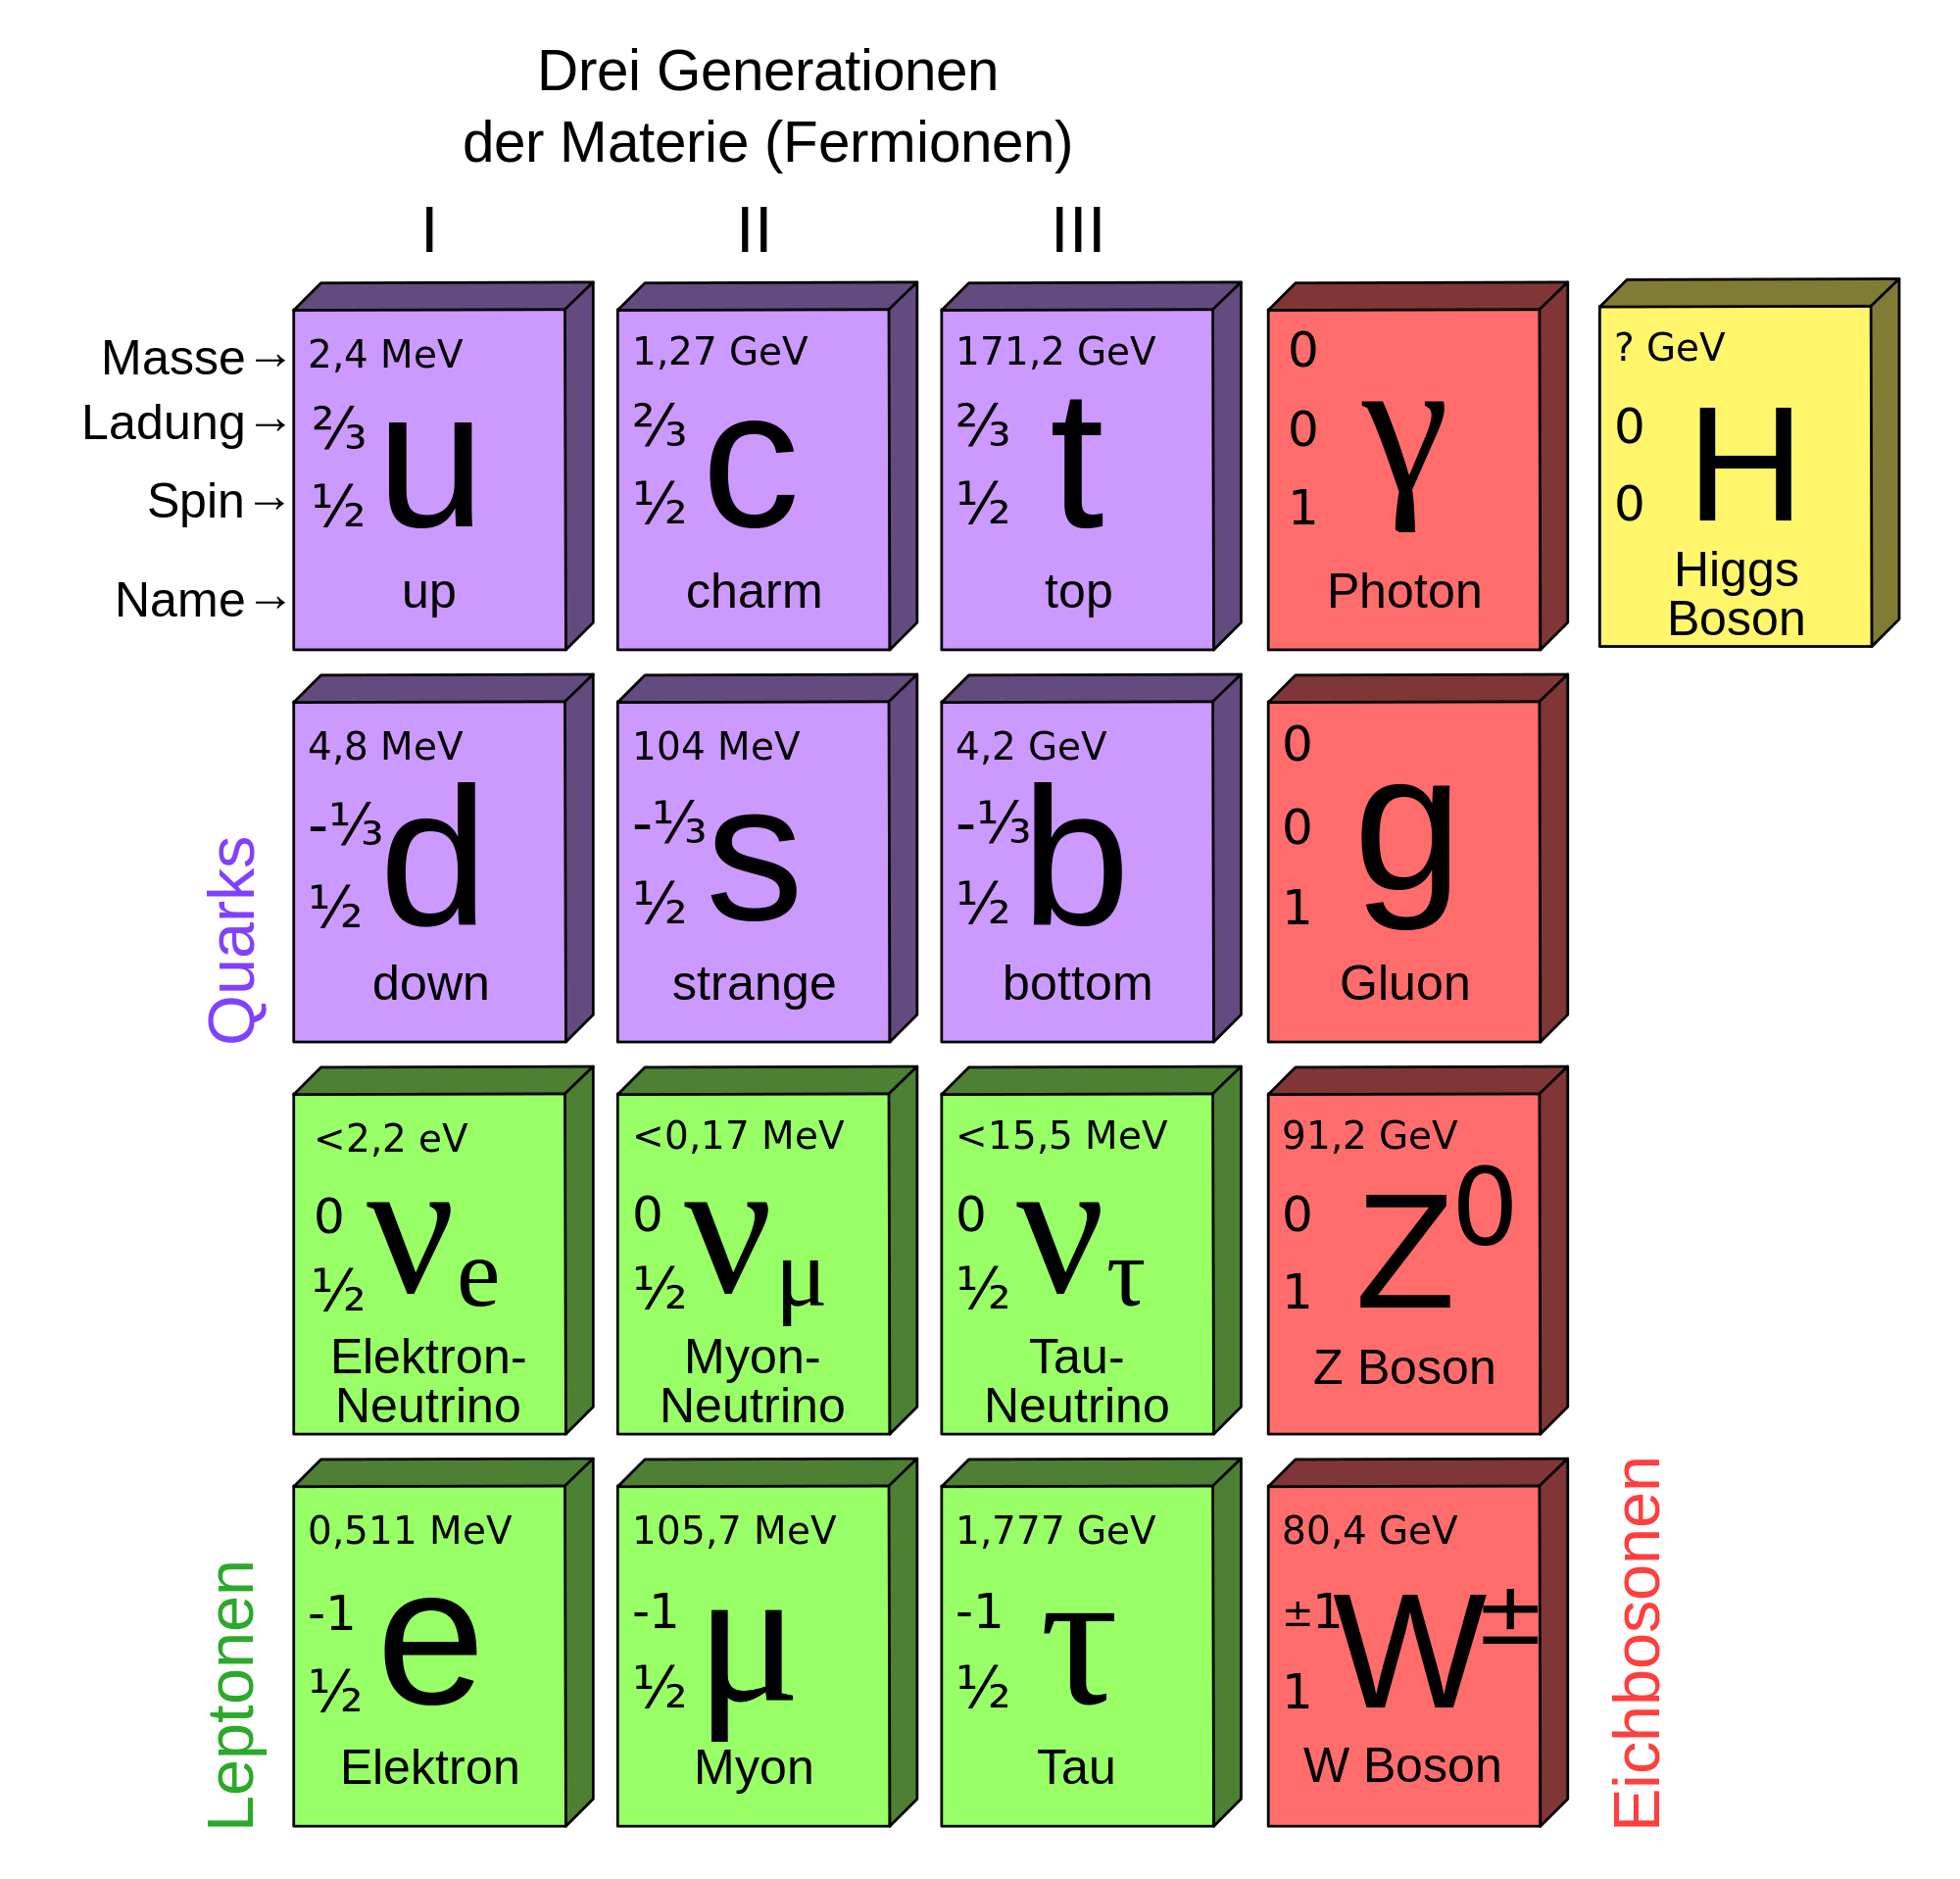
\includegraphics[width=0.5\textwidth]{standardmodell}
\caption{Das Standardmodell der Teilchenphysik \cite{wiki_standard}}
\label{fig:standardmodell}
\end{figure}

\subsection{B-Mesonen und ihre Mischung}
Mesonen sind Paare aus Quarks und Antiquarks beliebigen Flavours. B-Mesonen insbesondere bestehen aus einem Anti-b-Quark ($\mathrm{\overline{b}}$) mit einem u-, d-, c- oder s-Quark beziehungsweise aus der Kombination der jeweiligen Antiteilchen (Anti-B-Mesonen).

Die in dieser Arbeit betrachteten \Bd-Mesonen haben demnach die Quarkzusammensetzung $\Ket{\text{\Bd}} = \Ket{\overline{b}d}$ und sind elektrisch neutral. Solch neutrale Mesonen besitzen die Eigenschaft, dass sie sich in ihre Antiteilchen wandeln können und umgekehrt. Es findet folglich eine Oszillation zwischen \Bd und \Bdbar statt, die man auch Mischung nennt. Abbildung \ref{fig:bmixing} zeigt zwei mögliche Feynmangraphen für diesen Prozess. Innerhalb der Schleifen kann die Energieerhaltung kurzzeitig verletzt werden, sodass auch kurzerhand die deutlich schweren top-Quarks enstehen können. Zu diesem Mischungsprozess leisten sie sogar einen dominanten Beitrag. Präzise Messungen der \Bd-Mischung erlauben Aussagen bspw. über die top-Masse und grenzen damit das Standardmodell ein, gleichzeitig erhofft man sich, durch noch präzisere Messungen Hinweise auf \glqq neue Physik\grqq zu finden, die sich dann in kleinsten Korrekturen innerhalb der Schleife bemerkbar machen würden.

\begin{figure}[hptb]
\centering
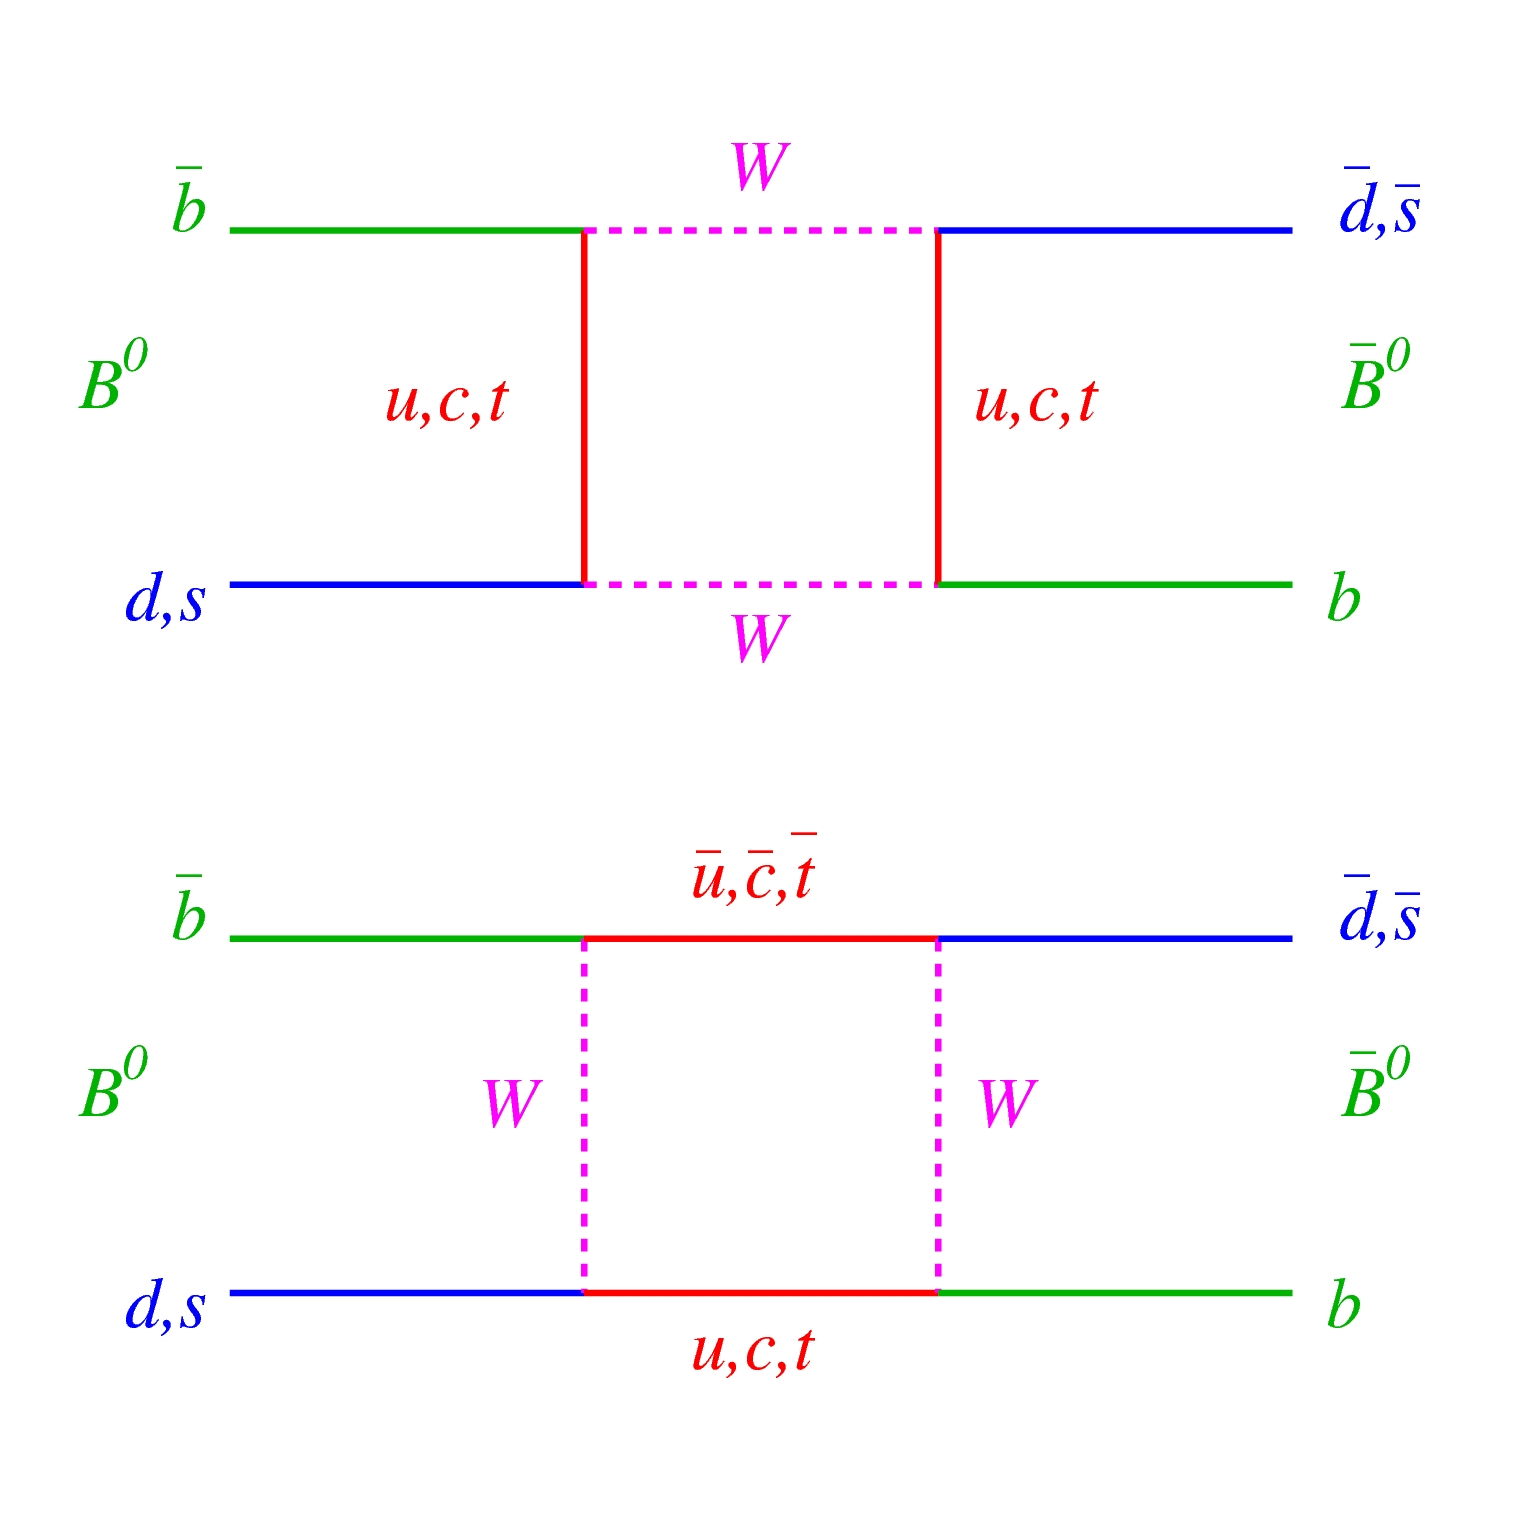
\includegraphics[width=0.5\textwidth]{bmixing}
\caption{Feynmangraphen zur Mischung von \Bd- und \Bdbar-Mesonen}
\label{fig:bmixing}
\end{figure}


\subsection{Der Zerfallskanal \Decaychannel}
In dieser Arbeit wird der Zerfallskanal \Decaychannel betrachtet. Abbildung \ref{fig:decay} zeigt entsprechende Feynmangraphen. Jener Kanal ist auch als \glqq goldener\grqq Zerfallskanal für die Messung der \CP-Verletzung bekannt. Hintergrund ist, dass der Endzustand $\Ket{\JPsi\Kshort}$ ein \CP-Eigenzustand ist ($\text{\CP}\Ket{\JPsi\Kshort} = - \Ket{\JPsi\Kshort}$). Die Teilchen $\JPsi$ und $\Kshort$ haben die Flavoureigenzustände $\Ket{\JPsi} = \Ket{c\overline{c}}$ sowie $\Ket{\Kshort} = \tfrac{1}{\sqrt{2}}\left(\Ket{d\overline{s}}-\Ket{s\overline{d}}\right)$. Diese Teilchen sind ebenfalls nicht stabil und zerfallen unter anderem weiter gemäß $\JPsi \rightarrow \mu^+\mu^-$ und $\Kshort \rightarrow \pi^+\pi^-$, was zur Rekonstruktion der \Bd-Mesonen im Detektor genutzt wird.

\begin{figure}[hptb]
\centering
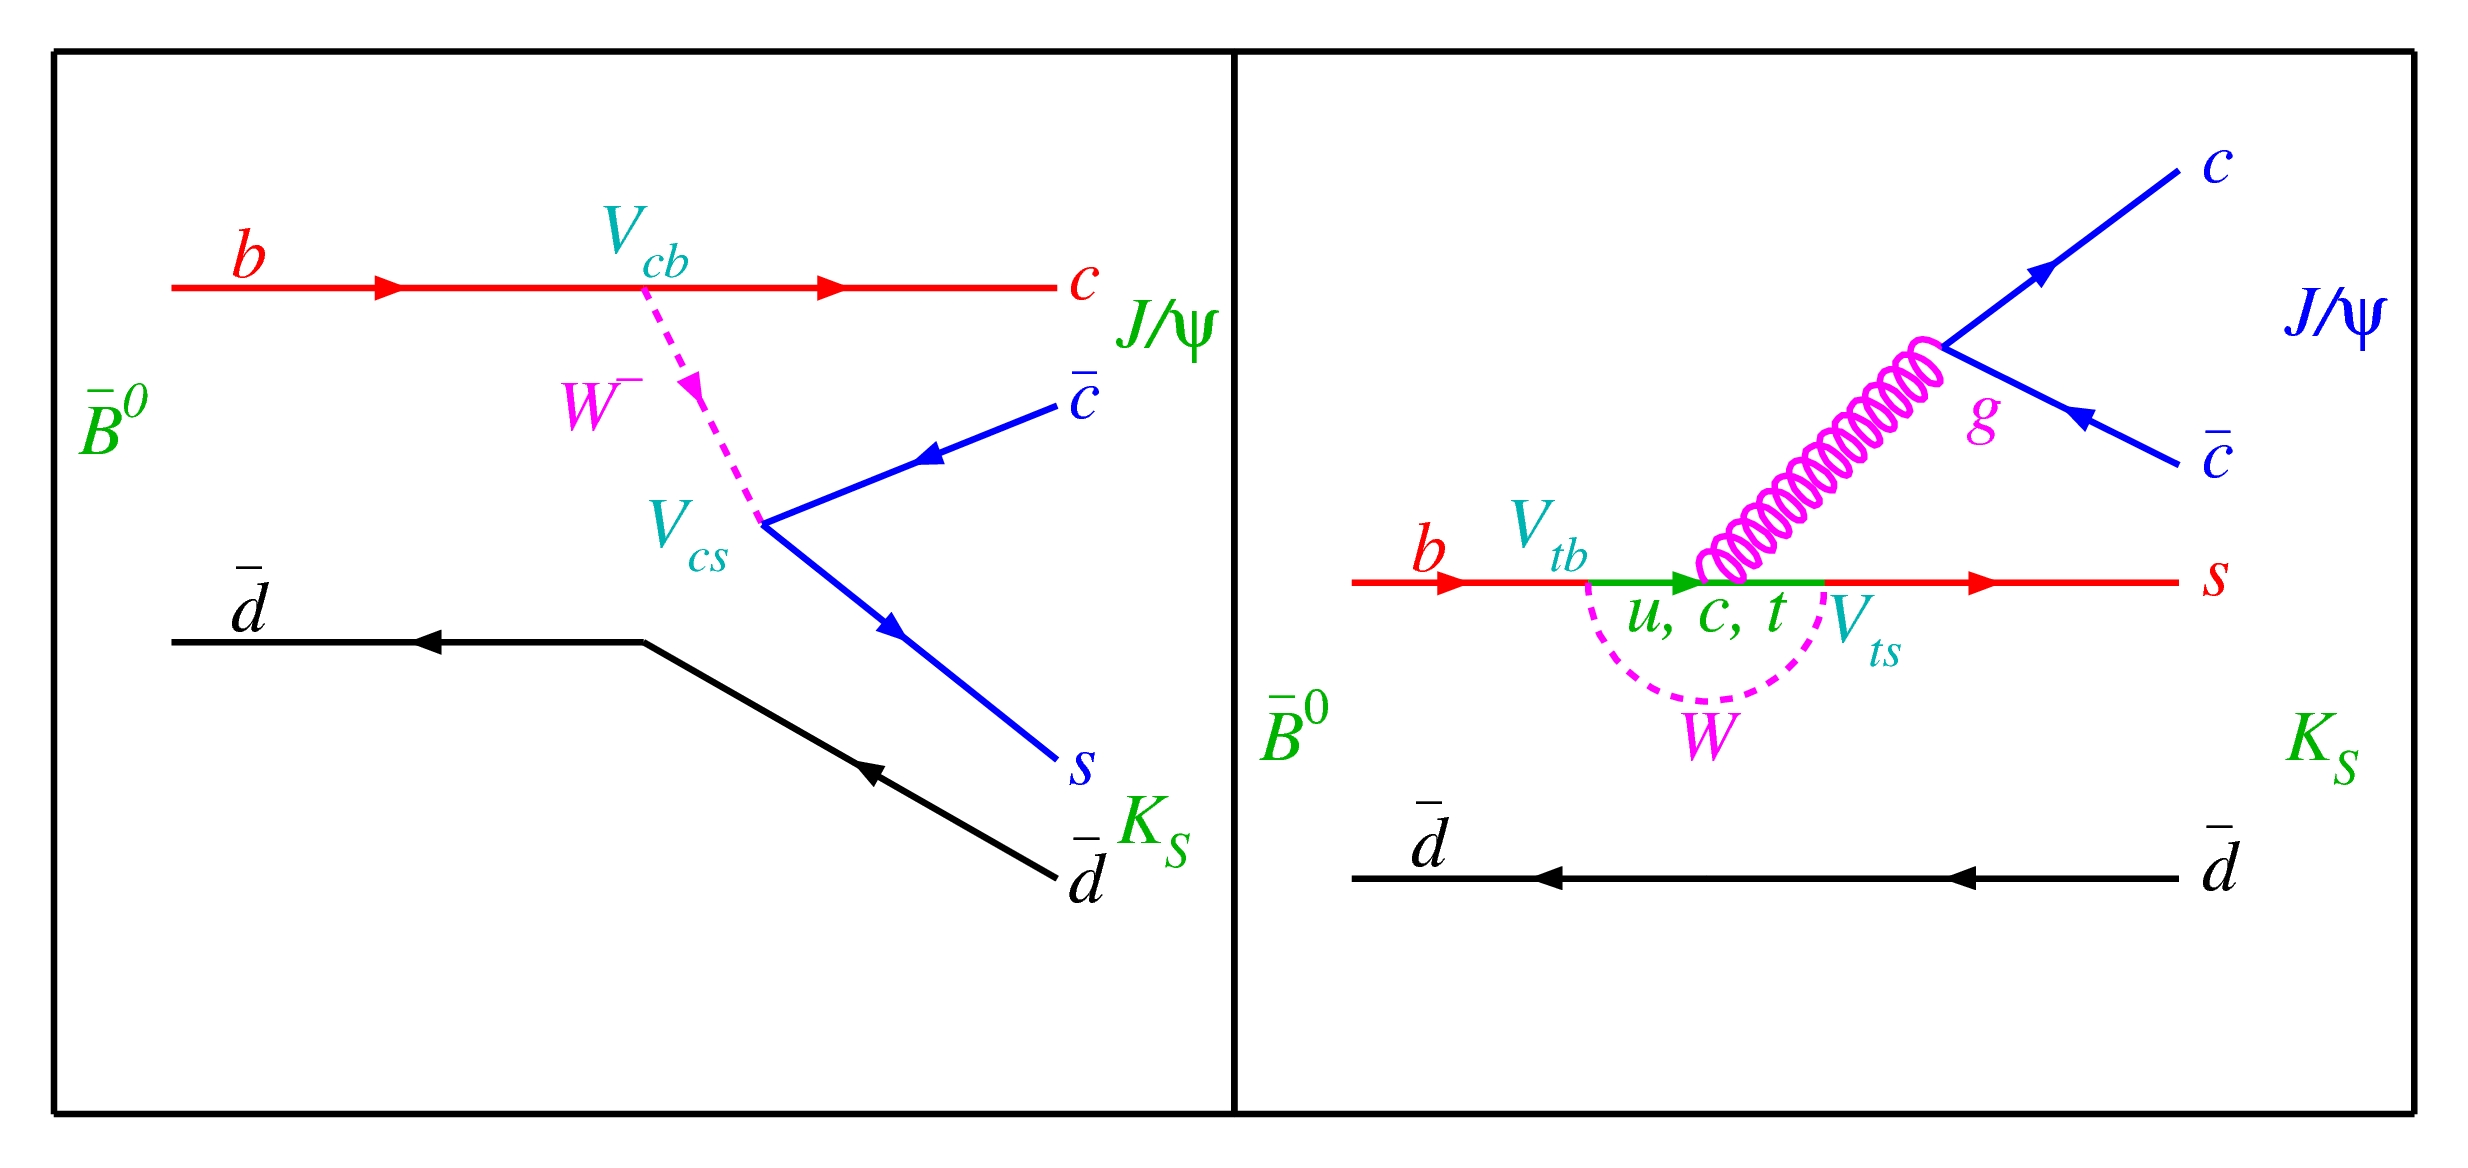
\includegraphics[width=\textwidth]{bd2jpsikshort}
\caption{Feynmangraph zum Zerfall \Decaychannel. Links: Baumdiagramm, rechts: Pinguindiagramm}
\label{fig:decay}
\end{figure}

\section{Diskrete Symmetrietransformationen}
Symmetrien sind in der Physik von zentraler Bedeutung. Gemäß dem Noether-Theorem existiert in der klassischen Physik zu jeder kontinuierlichen Symmetrie eine Erhaltungsgröße. In quantenmechanischen Systemen können wir drei diskrete Symmetrietransformationen betrachten:
\begin{enumerate}
\item \textbf{Parität $\mathcal{P}$:} \\
      Bei der Paritätsoperation wird das Vorzeichen der kartesischen Ortskoordinaten umgekehrt. Dies entspricht einer Punktspigelung.
\item \textbf{Ladungskonjugation $\mathcal{C}$:} \\
      Jedes Teilchen wird durch sein Antiteilchen ersetzt.
\item \textbf{Zeitumkehr $\mathcal{T}$:} \\
      Das Vorzeichen auf der Zeitachse wird umgekehrt. Da in der vorligenden Arbeit allerdings nur die CP-Verletzung gemessen werden soll, wird die Zeitumkehr im folgenden vernachlässigt.
\end{enumerate}
Entgegen der klassischen Intuition konnte Wu 1956 nachweisen, dass die Parität im $\beta$-Zerfall und damit in der schwachen Wechselwirkung nicht erhalten ist. Weitere Experimente zeigen, dass die schwache Wechselwirkung die Parität maximal verletzt: Neutrinos, die nur schwach wechselwirken können, sind stets \glqq linkshändig\grqq (Spin und Impuls antiparallel), Antineutrinos dagegen immer \glqq rechtshändig\grqq (Spin und Impuls parallel). Da der Spin im Gegensatz zum Impuls invariant unter $\mathcal{P}$-Transformation ist, würde diese Operation aus einem linkshändigen Neutrino ein rechtshändiges machen, was in der Nautr nicht realisiert ist.

Damit ist offensichtlich, dass die schwache Wechselwirkung auch die Ladungskonjugation verletzt: Wendet man die $\mathcal{C}$-Transformation auf ein linkshändiges Neutrino an, so erhält man ein linkshändiges Antineutrino. Dieses existiert aber wie bereits erwähnt nicht. Analog gilt die Überlegung auch für Antineutrinos.

\subsection{Scheinbare $\mathcal{CP}$-Invarianz}
Wendet man nun aber die Transformationen $\mathcal{P}$ und $\mathcal{C}$ direkt hintereinander an, so ergibt sich zunächst kein Widerspruch zur Natur (siehe Abb. \ref{fig:cp_invarianz}). Aus einen linkshändigen Neutrino wird ein rechtshändiges Antineutrino. Im Jahre 1964 wurde dann allerdings im Zerfall neutraler K-Mesonen erstmals $\mathcal{CP}$-Verletzung nachgewiesen. \cite{kleinknecht}

\begin{figure}[hptb]
\centering
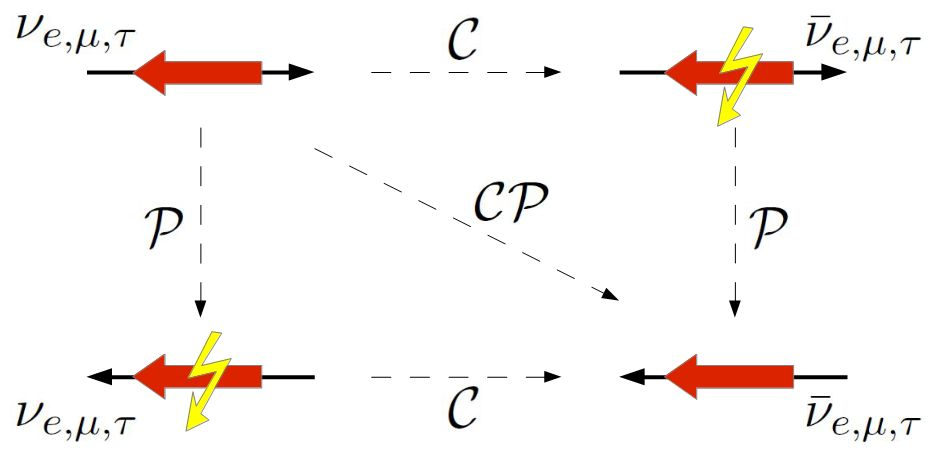
\includegraphics[width = 0.8\textwidth]{cp_invarianz}
\caption{Scheinbare $\mathcal{CP}$-Invarianz: Während eine reine $\mathcal{P}$- oder $\mathcal{C}$-Transformation zu in der Natur nicht realisierten Zuständen führt, scheint es bei der kombinierten $\mathcal{CP}$-Transformation keinen Widerspruch zu geben (dünne Pfeile: Impulsausrichtung, dicke Pfeile: Spinausrichtung).}
\label{fig:cp_invarianz}
\end{figure}



\section{\CP-Verletzung in der Mischung}
Die Flavoureigenzustände $\Ket{B^0} = \Ket{\overline{b}d}$ und $\Ket{\overline{B^0}} = \Ket{b\overline{d}}$ entsprechen nicht den Masseneigenzuständen. Wir definieren daher die normierten Zustände
\begin{align}
\Ket{B_h} = p \Ket{B^0} - q \Ket{\overline{B^0}} \label{eq:b_heavy}\\ 
\Ket{B_l} = p \Ket{B^0} + q \Ket{\overline{B^0}} \label{eq:b_light}\\
\text{mit} \quad |p|^2 + |q|^2 = 1
\end{align}
welche eine definierte Masse und Zerfallsbreite besitzen. Sie sind auch Eigenzustände eines nicht-hermiteschen Hamiltonoperators (Nichthermitizität wegen des möglichen Zerfalls der Teilchens). Dieser setzt sich zusammen aus den hermiteschen Massenoperatoren $M$ und $\Gamma$. Notieren wir die lineare Superposition der Zustände \ref{eq:b_heavy} und \ref{eq:b_light} als $\begin{pmatrix} p \\ q \end{pmatrix}$, so nimmt die zeitabhängige Schrödingergleichung die Form
\begin{align}
\im \diff{}{t}\begin{pmatrix} p \\ q \end{pmatrix} = \left(M - \frac{\im}{2} \Gamma\right) \begin{pmatrix} p \\ q \end{pmatrix}
\end{align}
an und führt zur folgenden zeitlichen Entwicklung der Zustände:
\begin{align}
\nonumber \Ket{B_{h/l}(t)} &= \e^{-\im m_{h/l}t-\frac{1}{2}\Gamma_{h/l}t}\Ket{B_{h/l}(0)} \\
                           &= \e^{-\gamma_{h/l}t}(p\Ket{B^0} \mp q\Ket{\overline{B^0}}) \\
&\text{mit} \quad \gamma_{h/l} = \im m_{h/l}+\frac{\Gamma_{h/l}}{2}
\end{align}
Hierbei ist $\gamma_{h/l}$ so definiert, dass $-\im\gamma_{h/l} = m_{h/l}-\frac{\im}{2}\Gamma_{h/l}$ die Eigenwerte des Hamiltonoperators $\mathcal{H} := \left(M - \frac{\im}{2} \Gamma\right)$ sind. Umgeschrieben auf die Flavoureigenzustände erhält man:
\begin{align}
\nonumber \Ket{B^0(t)} &= \frac{1}{2p}\left(\Ket{B_h} + \Ket{B_l}\right) \\
                       &= \frac{1}{2}\left[ (\e^{-\gamma_h t}+\e^{-\gamma_l t})\Ket{B^0} - \frac{q}{p}(\e^{-\gamma_h t}-\e^{-\gamma_l t})\Ket{\overline{B^0}}\right] \label{eg:b(t)}
\end{align}
Die Wahrscheinlichkeit für den Übergang eines $\Ket{B^0}$ (zum Zeitpunkt $t=0$) in ein $\Ket{\overline{B^0}}$ beträgt:
\begin{align}
\nonumber P(B^0\rightarrow\overline{B^0})(t) &= |\Braket{\overline{B^0}|B^0(t)}|^2 \\
                                        &= \frac{1}{4} \left|\frac{q}{p}\right|^2 \left[\e^{-\Gamma_h t} + \e^{-\Gamma_l t} - 2\e^{-\frac{1}{2}(\Gamma_h + \Gamma_l) t}\cos(\Delta m_d t)\right] \\
&\text{mit} \quad \Delta m_d = m_h - m_l
\end{align}

Analog gilt für die Übergangswahrscheinlichkeit eines $\Ket{\overline{B^0}}$ in ein $\Ket{B^0}$:
\begin{align}
P(\overline{B^0}\rightarrow B^0)(t) = \frac{1}{4} \left|\frac{p}{q}\right|^2 \left[\e^{-\Gamma_h t} + \e^{-\Gamma_l t} - 2\e^{-\frac{1}{2}(\Gamma_h + \Gamma_l) t}\cos(\Delta m_d t)\right] 
\end{align}

Es kommt daher in der Mischung zur \CP-Verletzung, wenn die Oszillation ungleichmäßig verläuft, anders ausgedrückt:
\begin{align}
\text{\CP-Verletzung in der Mischung} \qquad \Longleftrightarrow \qquad \left|\frac{p}{q}\right| \neq 1 
\end{align}

\section{Direkte \CP-Verletzung}
Die Zerfallsamplituden der neutralen $B^0$-Mesonen in einen Endzustand $\Ket{f}$ bzw. seinen \CP-konjugierten Zustand $\Ket{\overline{f}}$ sind definiert als
\begin{alignat}{2}
\nonumber A_f &= \Braket{f|\mathcal{H}|B^0}, && \qquad A_{\overline{f}} = \Braket{\overline{f}|\mathcal{H}|B^0}, \\
          \overline{A_f} &= \Braket{f|\mathcal{H}|\overline{B^0}}, && \qquad  \overline{A_{\overline{f}}} = \Braket{\overline{f}|\mathcal{H}|\overline{B^0}}. \label{eq:decay_amplitudes}
\end{alignat}
Dabei bezeichnet $\mathcal{H}$ einen Hamiltonoperator der schwachen Wechselwirkung. Ist \CP erhalten, dann sollten die Zerfallsraten, ergo auch die Zerfallsamplituden eines $B^0$ nach $f$ sowie eines $\overline{B^0}$ nach $\overline{f}$ gleich sein. Dies bedeutet:
\begin{align}
\text{Direkte \CP-Verletzung} \qquad \Longleftrightarrow \qquad \frac{|A_f|}{|\overline{A_{\overline{f}}}|} \neq 1 \quad \text{bzw.} \quad \frac{|\overline{A_f}|}{|A_{\overline{f}}|} \neq 1
\end{align}


\section{\CP-Verletzung in der Interferenz}
Die Zustände \ref{eq:b_heavy} und \ref{eq:b_light} haben eine nahezu gleiche Anzahl an Zerfällskanäle. Dies hat zur Folge, dass die Lebensdauern des schweren und leichten Zustands innerhalb weniger Prozent gleich sind:
\begin{align}
\Gamma := \Gamma_h = \Gamma_l \label{eq:Gamma}
\end{align}

Weiterhin sagt das Standard Modell nur eine kleine \CP-Verletzung in der \Bd - \Bdbar - Mischung voraus, sodass
\begin{align}
\left|\frac{p}{q}\right| = 1 \qquad \text{in} \mathcal{O}(10^{-3}). \label{eg:pq_approx}
\end{align}

Für das B-Meson-System bleibt daher nur die Möglichkeit der \CP-Verletzung in der Interferenz von Mischung und direktem Zerfall. Der in dieser Arbeit betrachtete Zerfallskanal $B_d^0 \rightarrow J/\Psi K_s^0$ hat einen \CP-Eigenzustand als Endzustand (\CP $\Ket{\JPsi\Kshort} = -\Ket{\JPsi\Kshort}$). In Anlehnung an \ref{eq:decay_amplitudes} sind die Zerfallsamplituden hier definiert als
\begin{align}
\nonumber A_f := \Braket{f|B^0(t)}, \qquad \overline{A_{f}} := \Braket{f|\mathcal{H}|\overline{B^0}}
\end{align}

Mit Blick auf die Zerfallsamplituden der Masseneigenzustände wird die komplexe Größe
\begin{align}
\lambda_f := \frac{q\overline{A_f}}{pA_f} \label{eq:lambda}
\end{align}
definiert. Ausgehend von Gleichung \ref{eg:b(t)} sowie mit Hilfe fer Gleichungen (\ref{eq:Gamma}), (\ref{eg:pq_approx}) und (\ref{eq:lambda}) gilt für die Zerfallsrate eines anfänglich reinen \Bd-Zustands:
\begin{align}
\nonumber \Gamma (B^0 \rightarrow \JPsi\Kshort) &= \frac{1}{4}\left| (\e^{-\gamma_h t}+\e^{-\gamma_l t})A_f - \frac{q}{p}(\e^{-\gamma_h t}-\e^{-\gamma_l t})\overline{A_f}\right|^2 \\
&= \frac{1}{2} \left|A_f\right|^2\e^{-\Gamma t} \left[1+|\lambda_f|^2 + (1-|\lambda_f|^2)\cos(\Delta m_d t) - 2\mathrm{Im}(\lambda_f)\sin(\Delta m_d t)\right]
\end{align}
Analog:
\begin{align}
\Gamma (\overline{B^0} \rightarrow \JPsi\Kshort) &= \frac{1}{2} \left|A_f\right|^2\e^{-\Gamma t} \left[1+|\lambda_f|^2 -(1-|\lambda_f|^2)\cos(\Delta m_d t) + 2\mathrm{Im}(\lambda_f)\sin(\Delta m_d t)\right]
\end{align}

Damit kann die vom Standard Modell prognostizierte \CP-verletzende Asymmetrie 
\begin{align}
\mathcal{A}_{\text{\CP}} &= \frac{\Gamma (\overline{B^0} \rightarrow \JPsi\Kshort) - \Gamma (B^0 \rightarrow \JPsi\Kshort)}{\Gamma (\overline{B^0} \rightarrow \JPsi\Kshort) + \Gamma (B^0 \rightarrow \JPsi\Kshort)} \\
&= -\frac{1-|\lambda_f|^2}{1+|\lambda_f|^2}\cos(\Delta m_d t) + \frac{2\mathrm{Im}(\lambda_f)}{1+|\lambda_f|^2}\sin(\Delta m_d t) \\
&=: \CJPsi \cos(\Delta m_d t) + \SJPsi \sin(\Delta m_d t)
\end{align}
berechnet werden und vereinfacht sich - da $\Ket{\JPsi\Kshort}$ ein \CP-Eigenzustand ist, gilt $|\lambda_f| = 1$ - hier zu
\begin{align}
\mathcal{A}_{\text{\CP}} = \mathrm{Im}(\lambda_f)\sin(\Delta m_d t) .
\end{align}

Damit kann im B-Meson-System, insbesondere im Zerfall $B_d^0 \rightarrow J/\Psi K_s^0$ durch Messung der Asymmetrie-Amplitude $\SJPsi$ \CP-Verletzung in der Interferenz gemessen werden.

\begin{align}
\text{\CP-Verletzung in der Interferenz} \qquad \Longleftrightarrow \qquad \SJPsi = \mathrm{Im}(\lambda)\neq 0
\end{align}

\section{CKM-Formalismus}
Durch Austausch eines W$^{\pm}$-Bosons können Quarks ihren Flavour ändern. Dabei sind sie aber nicht an ihre jeweilige Generation gebunden, sondern können - wenn auch zum Teil stark unterdrückt - prinzipiell den Flavour einer jeden Generation annehmen. Ein kleines Beispiel: Der Eigenzustand $\Ket{u}$ der starken Wechselwirkung geht über den schwachen Prozess (Austausch eines W$^{\pm}$-Bosons) nicht in ein $\Ket{d}$ über, sondern vielmehr in eine Linearkombination aus $\Ket{d}$, $\Ket{s}$ und $\Ket{b}$, die im folgenden mit $\Ket{d'}$ bezeichnet wird. Allgemein werden die möglichen Linearkombinationen durch die Cabibbo-Kobayashi-Maskawa-Matrix (kurz: CKM-Matrix) beschrieben.
\begin{align}
\begin{pmatrix}
\Ket{d'} \\ \Ket{s'} \\ \Ket{b'}
\end{pmatrix}
=
\begin{pmatrix}
V_{ud} & V_{us} & V_{ub} \\
V_{cd} & V_{cs} & V_{cb} \\
V_{td} & V_{ts} & V_{tb} \\
\end{pmatrix}
\cdot
\begin{pmatrix}
\Ket{d} \\ \Ket{s} \\ \Ket{b}
\end{pmatrix}
\end{align}

Das Betragsquadrat eines jeden Matrixelementes $|V_{ij}|^2$ gibt dabei die Wahrscheinlichkeit für den Übergang eines Quarks $\Ket{i}$ in ein $\Ket{j}$ an. Da die $V_{ij}$ prinzipiell komplex sein können, gibt es zunächst 18 freie Parameter, die zu bestimmen sind. Diese Zahl reduziert sich zum einen um 5 relative Quarkphasen, die physikalisch nicht beobachtbar sind. Zum anderen reduziert die Forderung nach Unitarität der CKM-Matrix die Zahl der unabhängigen Parameter um 9, sodass am Ende 4 Parameter, 3 Euler Winkel sowie eine Phase, welche für die \CP-Verletzung verantwortlich ist, zu bestimmen sind. Die CKM-Matrix lässt sich näherungsweise durch die Wolfenstein-Parametrisierung darstellen:

\begin{align}
V_{\text{CKM}}=
\begin{pmatrix}
V_{ud} & V_{us} & V_{ub} \\
V_{cd} & V_{cs} & V_{cb} \\
V_{td} & V_{ts} & V_{tb} \\
\end{pmatrix}
=
\begin{pmatrix}
1-\frac{\lambda^2}{2} & \lambda & A\lambda^3(\rho-\im\eta) \\
-\lambda & 1-\frac{\lambda^2}{2} & A\lambda^2 \\
A\lambda^3(1-\rho-\im\eta) & -A\lambda^2 & 1
\end{pmatrix}
+ \mathcal{O}(\lambda^4)
\end{align}

Für den Zerfall von \Bd-Mesonen ist die Unitaritätsbedingung
\begin{align}
V_{ud}V_{ub}^* + V_{cd}V_{cb}^* + V_{td}V_{tb}^* = 0
\end{align}
von besonderer Bedeutung. Man kann die einzelnen Summanden nun in der $(\rho,\eta)$-Ebene auftragen und erhält dabei ein sogenanntes Unitaritätsdreieck. Es wird so normiert, dass die Unterseite bei (0,0) beginnt und bei (1,0) endet (siehe Abb. \ref{fig:unitarity}). Die obere Ecke liegt dann bei $(\overline{\rho}, \overline{\eta})$, wobei $\overline{\rho} = \rho(1-\lambda^2/2)$ und $\overline{\eta} = \eta(1-\lambda^2/2)$ gemäß der Wolfenstein-Parametrisierung sind. Die Winkel des Dreiecks erhält man über
\begin{align}
\alpha = \text{arg}\left[-\frac{V_{td}V_{tb}^*}{V_{ud}V_{ub}^*}\right], \qquad
\beta = \text{arg}\left[-\frac{V_{cd}V_{cb}^*}{V_{td}V_{tb}^*}\right], \qquad
\gamma = \text{arg}\left[-\frac{V_{ud}V_{ub}^*}{V_{cd}V_{cb}^*}\right].
\end{align}

\begin{figure}[hptb]
\centering
%\includegraphics[width=\textwidth]{•}
\caption{Unitaritätsdreieck}
\label{fig:unitarity}
\end{figure}

Das Standardmodell stellt für den hier untersuchten Zerfallskanal eine Beziehung zwischen dem Winkel $\beta$ und der komplexen Größe $lambda_f$ aus Gleichung \ref{eq:lambda} her (\cite{nir}, \cite{noguchi}):
\begin{align}
&\lambda_f = \underbrace{\frac{V_{td}V_{tb}^*}{V_{td}^*V_{tb}}}_{\frac{q}{p}} \underbrace{\frac{V_{cd}^*V_{cb}}{V_{cd}V_{cb}^*}}_{\frac{\overline{A_f}}{A_f}} = \e^{2\im\beta} \\
\Longrightarrow &\SJPsi = \mathrm{Im}(\lambda_f) = \sin(2\beta).
\end{align}
 
Durch Messung der Amplitude der \CP-Asymmetrie kann man direkte Rückschlüsse auf den CKM-Winkel $\beta$ ziehen.

\chapter{Datenselektion}

\chapter{Analyse / Fit}
\section{Fitmethode SFit}
\section{Wahrscheinlichkeitsdichtefunktion}
\begin{equation}
xxx     \label{eg:fit_pdf}
\end{equation}
\section{Fitergebnis} \label{kap:fitergebnis}
Wir erhalten schließlich:
\begin{align}
\SJPsi = xxx \pm xxx     \label{eq:fit_result}
\end{align}

\chapter{Abschätzung systematischer Unsicherheiten} \label{kap:systematik}
Der Fitter liefert zwar eine statistische Unsicherheit auf $\SJPsi$, allerdings ist eine Betrachtung der Systematik unerlässlich. Im Folgenden wird daher der Einfluss einiger Effekte auf das Fitergebnis untersucht und anschließend der systematische Fehler abgeschätzt.

\section{Fitmethode} \label{kap:fit_bias}
Es ist allgemein bekannt, dass die Parameterabschätzung der Maximum-Like\-li\-hood-Methode für eine große Zahl an Messwerten gegen den \glqq wahren Wert\grqq\ konvergiert, für wenig Statistik verfälscht sie jedoch das Ergebnis - sie produziert ein sogenanntes Bias. Um abzuschätzen, ob und in welchem Maße es zu einem Bias kommt, wird eine Toy Monte Carlo - Studie (kurz: Toy MC) durchgeführt. Dabei werden zufällig Daten der Massen- und Eigenzeit-WDF aus Gleichung (\ref{eq:pdf_masse}) bzw. (\ref{eq:fit_pdf}) folgend mit den gewünschten Parametern generiert und im Anschluss gefittet. Zur Generation der Massen- und Eigenzeitverteilung werden die aus den Fits erhaltenen Parameter verwendet (siehe Tabellen \ref{tab:fit_masse} und \ref{tab:fit_results}). Die einzige Ausnahme bildet $\SJPsi$, da diese zum Zeitpunkt dieser Studie noch verdeckt war. Hier wurde mit $\SJPsi = 0,72$, dem Resultat der Analyse aus 2011 \cite{lhcb-paper}, generiert. Entsprechend der Statistik im verwendeten Datensatz werden hier jeweils 20000 Ereignisse generiert. Durch mehrmaliges Wiederholen von Generation und Fit sollten die gefitteten Parameter am Ende mit der Größe des statistischen Fehlers gaußverteilt um die in der Generation verwendeten Parameter sein. Kommt es zu Abweichungen davon, so ist dies auf die Fitmethode oder eine fehlerhafte Implementation des Experimentators zurückzuführen. Um statistisch zuverlässige Aussagen treffen zu können, wurden in dieser Toy MC - Studie insgesamt 20000 Wiederholungen durchgeführt.

\begin{figure}[hptb]
\centering
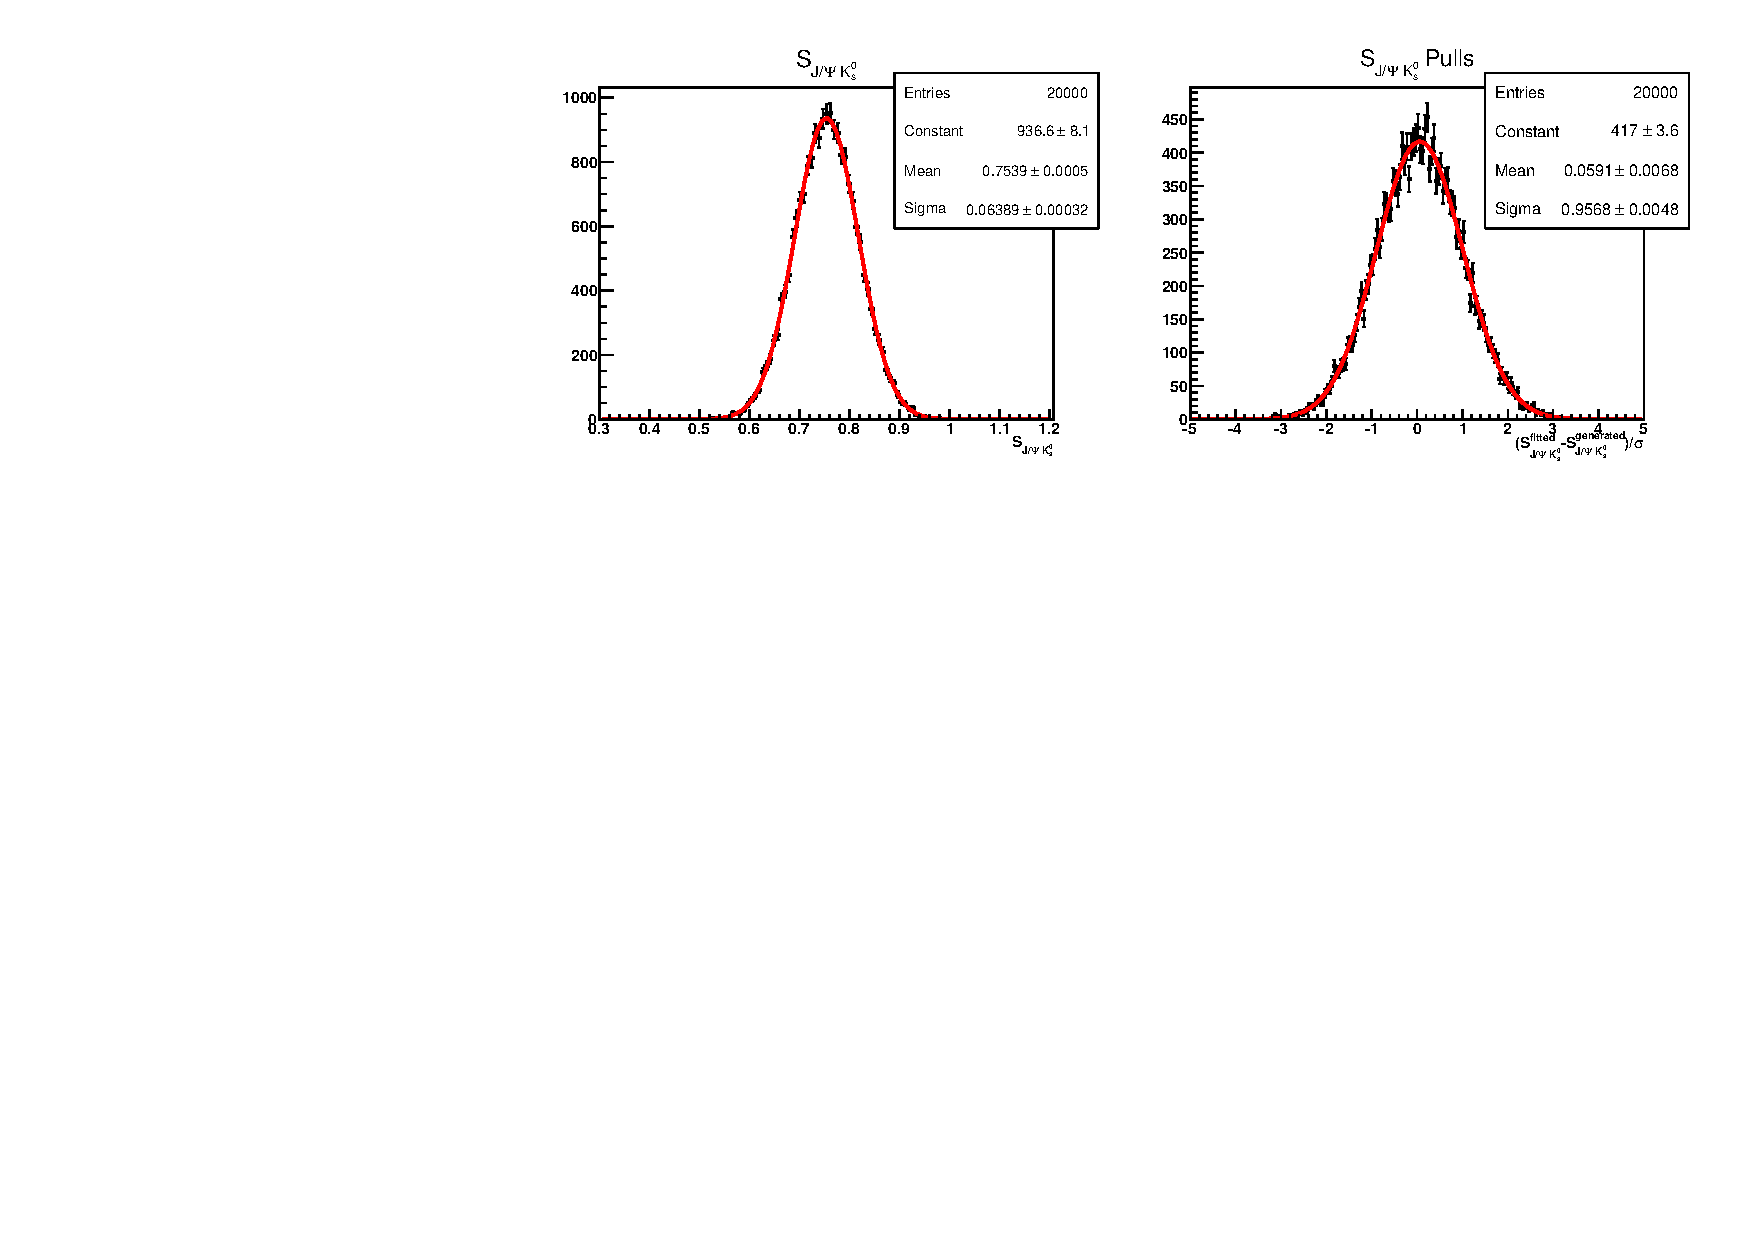
\includegraphics[width = \textwidth]{fit_bias}
\caption{Verteilung der aus der Toy MC Studie erhaltenen Amplituden $\SJPsi$ (links) sowie die dazugehörigen Pulls (rechts)}
\label{fig:fit_bias}
\end{figure}

Abbildung \ref{fig:fit_bias} zeigt sowohl die Verteilung der gefitteten Amplitude $\SJPsi$ als auch die Pulls, die sich mittels $(\SJPsi^{\text{gefittet}} - \SJPsi^{\text{generiert}})/\sigma^{\text{gefittet}}$ berechnen lassen. Der Mittelwert der Amplitudenverteilung (links) $\SJPsi^{\text{ToyMC}} = 0,7234 \pm 0,0004$ weicht signifikant vom generierten Wert $\SJPsi = 0,7200$ ab, es gibt also ein Bias. An der Pull-Verteilung lassen sich prinzipiell zwei Dinge beobachten:
\begin{enumerate}
    \item An der Verschiebung des Pull-Mittelwertes $\mu = 0,0522 \pm 0,0067$ von der Null sieht man deutlich, dass es - wie bereits erwähnt - ein kleines, aber signifikantes Bias gibt. Indem dieses Bias mit der statistischen Unsicherheit aus dem Fitergebnis (siehe Gl. (\ref{eq:fit_result})) multipliziert wird, erhält man eine Abschätzung der aus der Fitmethode resultierenden Unsicherheit:
        \begin{align}
        \delta\SJPsi^{Fit} = 0,0522 \cdot 0,0626 = 0,0033
        \end{align}

    \item Mit einem $\sigma = 0,941 \pm 0,005$ ist die Pull-Verteilung signifikant zu schmal. Bei einer zufälligen Streuung der Werte wird $\sigma=1$ erwartet. Dies bedeutet, dass der Fit den statistischen Fehler um $5,9\%$ überschätzt. Jenes Ergebnis kann später als Faktor zur Korrektur des statistischen Fehlers verwendet werden. 
\end{enumerate}

\subsubsection{Ursachen des Bias und der Fehlerüberschätzung}
Es bleibt zu klären, welche Ursachen zu dem Bias und der Fehlerüberschätzung führen. Wie bereits erwähnt, verfälscht die Likelihood-Methode für zu wenige Messwerte / Ereignisse die Parameterabschätzung. Demnach liegt die Vermutung nahe, dass im vorliegenden Datensatz zu wenig Ereignisse (\glqq Statistik\grqq) vorhanden sind. Daher wurden weitere Toy MC Studien mit unterschiedlicher Anzahl an generierten Teilchen pro Toy durchgeführt. Die Ergebnisse sind in Tabelle \ref{tab:fit_bias_events} aufgeführt und in Abbildung \ref{fig:fit_bias_events} nochmals visualisiert. Man sieht, dass das Bias mit erhöhter Statistik deutlich reduziert wird und damit zu wenig Statistik als Hauptursache hierfür angesehen werden kann.
\begin{table}[hptb]
\centering
\caption{Toy MC Studien mit unterschiedlicher Anzahl an generierten Ereignissen pro Toy. Genannt wird der Mittelwert $\mu$ der $\SJPsi$-Pull-Verteilung.}
\label{tab:fit_bias_events}
\begin{tabular}{cr@{$\pm$}l}
\hline \hline 
Teilchen pro Toy & \multicolumn{2}{c}{$\mu$}  \\ \hline
20000            &  0,0522 & 0,0067 \\
50000            &  0,0358 & 0,0067 \\
100000           &  0,0257 & 0,0068 \\
200000           &  0,0145 & 0,0068 \\ 
\hline \hline
\end{tabular}
\end{table}
\begin{figure}[hptb]
\centering
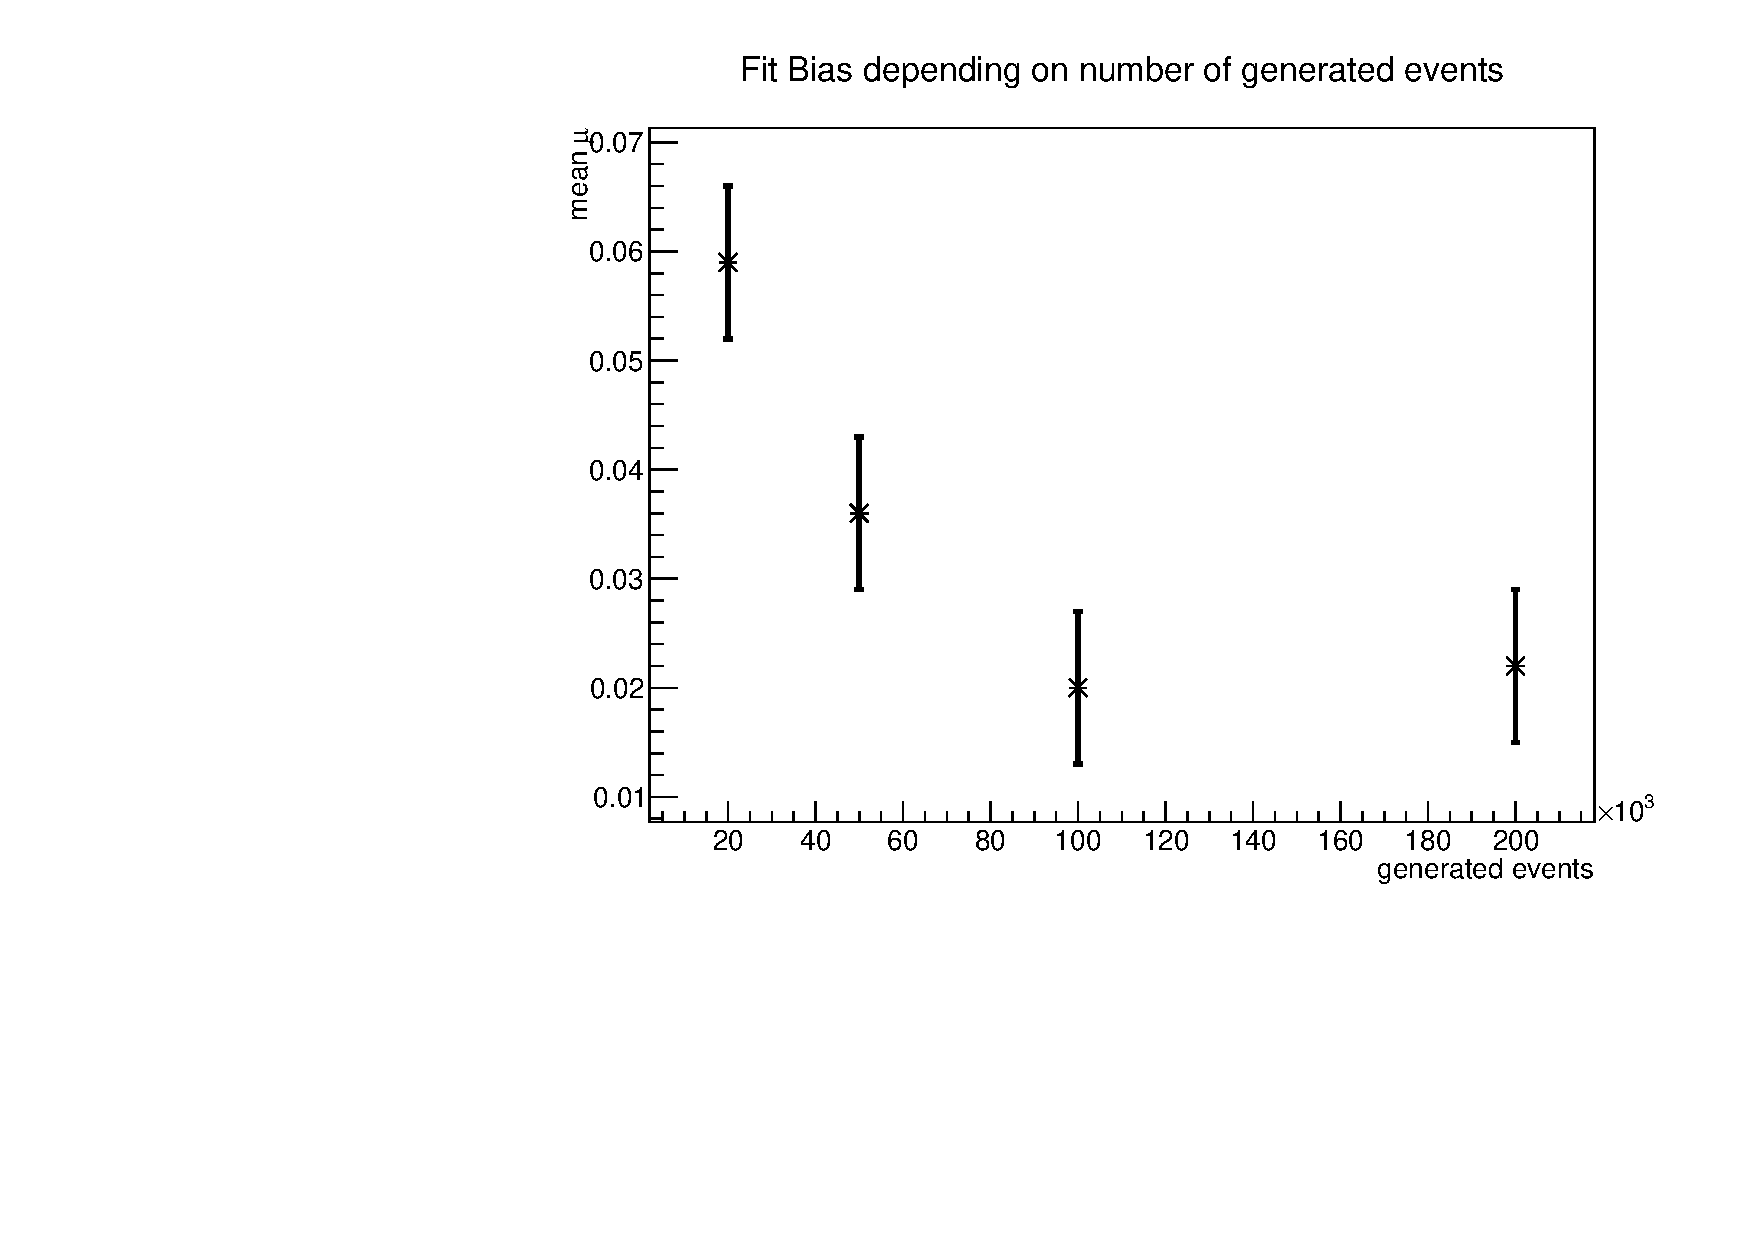
\includegraphics[width=\textwidth]{fit_bias_statistics}
\caption{Toy MC Studien mit unterschiedlicher Anzahl an generierten Ereignissen pro Toy. Als Maß für das Fit Bias dient der Mittelwert $\mu$ der $\SJPsi$-Pull-Verteilung. Der erste Eintrag entspricht der in Daten vorliegenden Statistik.}
\label{fig:fit_bias_events}
\end{figure}

Die Fehlerüberschätzung tritt auf, sobald man in den Toys Untergrund miteinbezieht (ohne Untergrund erhält man ein $\sigma=1,007\pm 0,005$ und ist damit kompatibel zur Eins). Es ist bekannt, dass die verwendete sFit-Methode die Fehlerpropagation (gerade bei Untergrund) nicht korrekt ausführt. Es wurde zuvor eine Fehlerkorrektur implementiert, dabei handelt es sich jedoch um eine Näherung. Für eine tiefergehende Studie müsste die Fehlerkorrektur entsprechend analysiert werden.

\section{Kalibration der Flavour Tagging Algorithmen} \label{kap:syst_tagging}
Im Fit werden bei den Parametern der Tagging Kalibration durch gaußische Einschränkung der Parameter deren statistische Fehler berücksichtigt. Bislang unbeachtet blieben die systematischen Fehler von $p_0$ und $p_1$, deren Einfluss im Folgenden untersucht wird. Leider sind die externen Studien zur Systematik des in dieser Analyse verwendeten Flavour Taggings noch nicht abgeschlossen, sodass die systematischen Fehler $\delta p_0^{\text{stat.}}$ sowie $\delta p_1^{\text{stat.}}$ noch nicht vorliegen. Um dennoch ein Gefühl für den Einfluss des Flavour Taggings zu bekommen, werden die systematischen Fehler der 2011-Analyse \cite{lhcb-paper} herangezogen. Die Annahme und Erwartung ist, dass sich die Systematiken zwischen 2011 und 2012 kaum unterscheiden. Für eine endgültige Analyse muss dieser Schritt jedoch wiederholt werden, sobald die Analyse des Flavour Taggings aus 2012 abgeschlossen ist. Eine weitere Möglichkeit wäre dann, die Parameter im Eigenzeitfit mit $\sigma = \sqrt{\sigma_{\text{stat.}}^2+\sigma_{\text{syst.}}^2}$ gaußisch einzuschränken und beide Unsicherheiten auf diese Weise zu berücksichtigen. In dieser Arbeit werden nun folgende Werte und Fehler der Kalibrationsparameter $p_0$ und $p_1$ verwendet:
\begin{align}
p_0 &= 0,382 \pm 0,003\ \text{(stat.)} \pm 0,008\ \text{(syst.)}, \\
p_1 &= 0,981 \pm 0,024\ \text{(stat.)} \pm 0,012\ \text{(syst.)}.
\end{align}

\subsubsection{Variation der Parameter in den Daten}
Einen ersten Überblick über die Systematik erhält man, indem man
im regulären Eigenzeitfit die Startwerte der Parameter $p_0$ und $p_1$ um ihre systematischen Fehler variiert. In allen vier möglichen Kombinationen wird der systematische Fehler auf $p_0$ und $p_1$ addiert bzw. subtrahiert, dann der Fit durchgeführt und schließlich die Abweichung vom regulären Fitergebnis für $\SJPsi$ berechnet. Der verdeckte Referenzwert aus dem Fit beträgt
\begin{align}
\SJPsi = 0,5347 \pm 0,0626.
\end{align}
\begin{table}[hptb]
\centering
\caption{Variation des Fitergebnisses für $\SJPsi$ bei Veränderung der Startwerte für $p_0$ und $p_1$ $\pm$ ihrer systematischen Unsicherheiten.}
\label{tab:syst_fit_calib_data}
$\begin{array}{cc|r@{\pm}l|r}
\hline\hline
p_0  &  p_1  &  \multicolumn{2}{c|}{\SJPsi}  & \Delta\SJPsi   \\ \hline
0,382 - 0,008  &  0,981 - 0,024  &  0,5109 & 0,0604  &  -0,0238 \\
0,382 - 0,008  &  0,981 + 0,024  &  0,5103 & 0,0604  &  -0,0244 \\
0,382 + 0,008  &  0,981 - 0,024  &  0,5599 & 0,0649  &   0,0252 \\
0,382 + 0,008  &  0,981 + 0,024  &  0,5591 & 0,0648  &   0,0244 \\
\hline\hline
\end{array}$
\end{table}
Die Ergebnisse sind Tabelle \ref{tab:syst_fit_calib_data} zu entnehmen. Die größte Abweichung beträgt hier $\Delta\SJPsi = 0,0252$.

\subsubsection{Variation der Parameter in Toy MC}
Eine präzisere Möglichkeit der Abschätzung besteht darin, sich entsprechende Toys mit verfälschten $p_0$ und $p_1$ zu generieren und diese dann normal zu fitten. Im Folgenden werden bei der Generation der Toys die Parameter $p_0$ und $p_1$ um ihre systematischen Unsicherheiten variiert, der Fit dann allerdings mit den ursprünglichen Parameterwerten durchgeführt. Als Referenzwert dient die Toy MC Studie aus Kapitel \ref{kap:fit_bias}, da dort mit den regulären Parametern $p_0$ und $p_1$ generiert und gefittet wurde. Jene Amplitude betrug
\begin{align}
\SJPsi = 0,7234 \pm 0,0004.
\end{align}
\begin{table}[hptb]
\centering
\caption{Variation des Fitergebnisses für $\SJPsi$ bei Veränderung der Parameterwerte $p_0$ und $p_1$ $\pm$ ihrer systematischen Unsicherheiten bei der Generation von Toys}
\label{tab:syst_fit_calib_toys}
$\begin{array}{cc|r@{\pm}l|r}
\hline\hline
p_0  &  p_1  &  \multicolumn{2}{c|}{\SJPsi}  & \Delta\SJPsi   \\ \hline
0,382 - 0,008  &  0,981 - 0,024  &  0,7515 & 0,0004  &   0,0281 \\
0,382 - 0,008  &  0,981 + 0,024  &  0,7565 & 0,0004  &   0,0331 \\
0,382 + 0,008  &  0,981 - 0,024  &  0,6909 & 0,0004  &  -0,0325 \\
0,382 + 0,008  &  0,981 + 0,024  &  0,6966 & 0,0004  &  -0,0244 \\
\hline\hline
\end{array}$
\end{table}

Die Ergebnisse sind Tabelle \ref{tab:syst_fit_calib_toys} zu entnehmen, die dazugehörigen Plots werden in Abbildung \ref{fig:toys_tag_calib} gezeigt. Die größte Abweichung beträgt hier $\Delta\SJPsi = 0,0331$ und ist auch größer als bei Variation der Parameter in den Daten. Dementsprechend wird der systematische Fehler durch die Flavour Tagging Kalibration mit ebendiesem Wert konservativ abgeschätzt:
\begin{align}
\delta\SJPsi^{\text{FTK}} = 0,0331.
\end{align}
\begin{figure}[hptb]
\centering
\subfigure[{$p_0 - \Delta p_0$,  $p_1 - \Delta p_1$}]{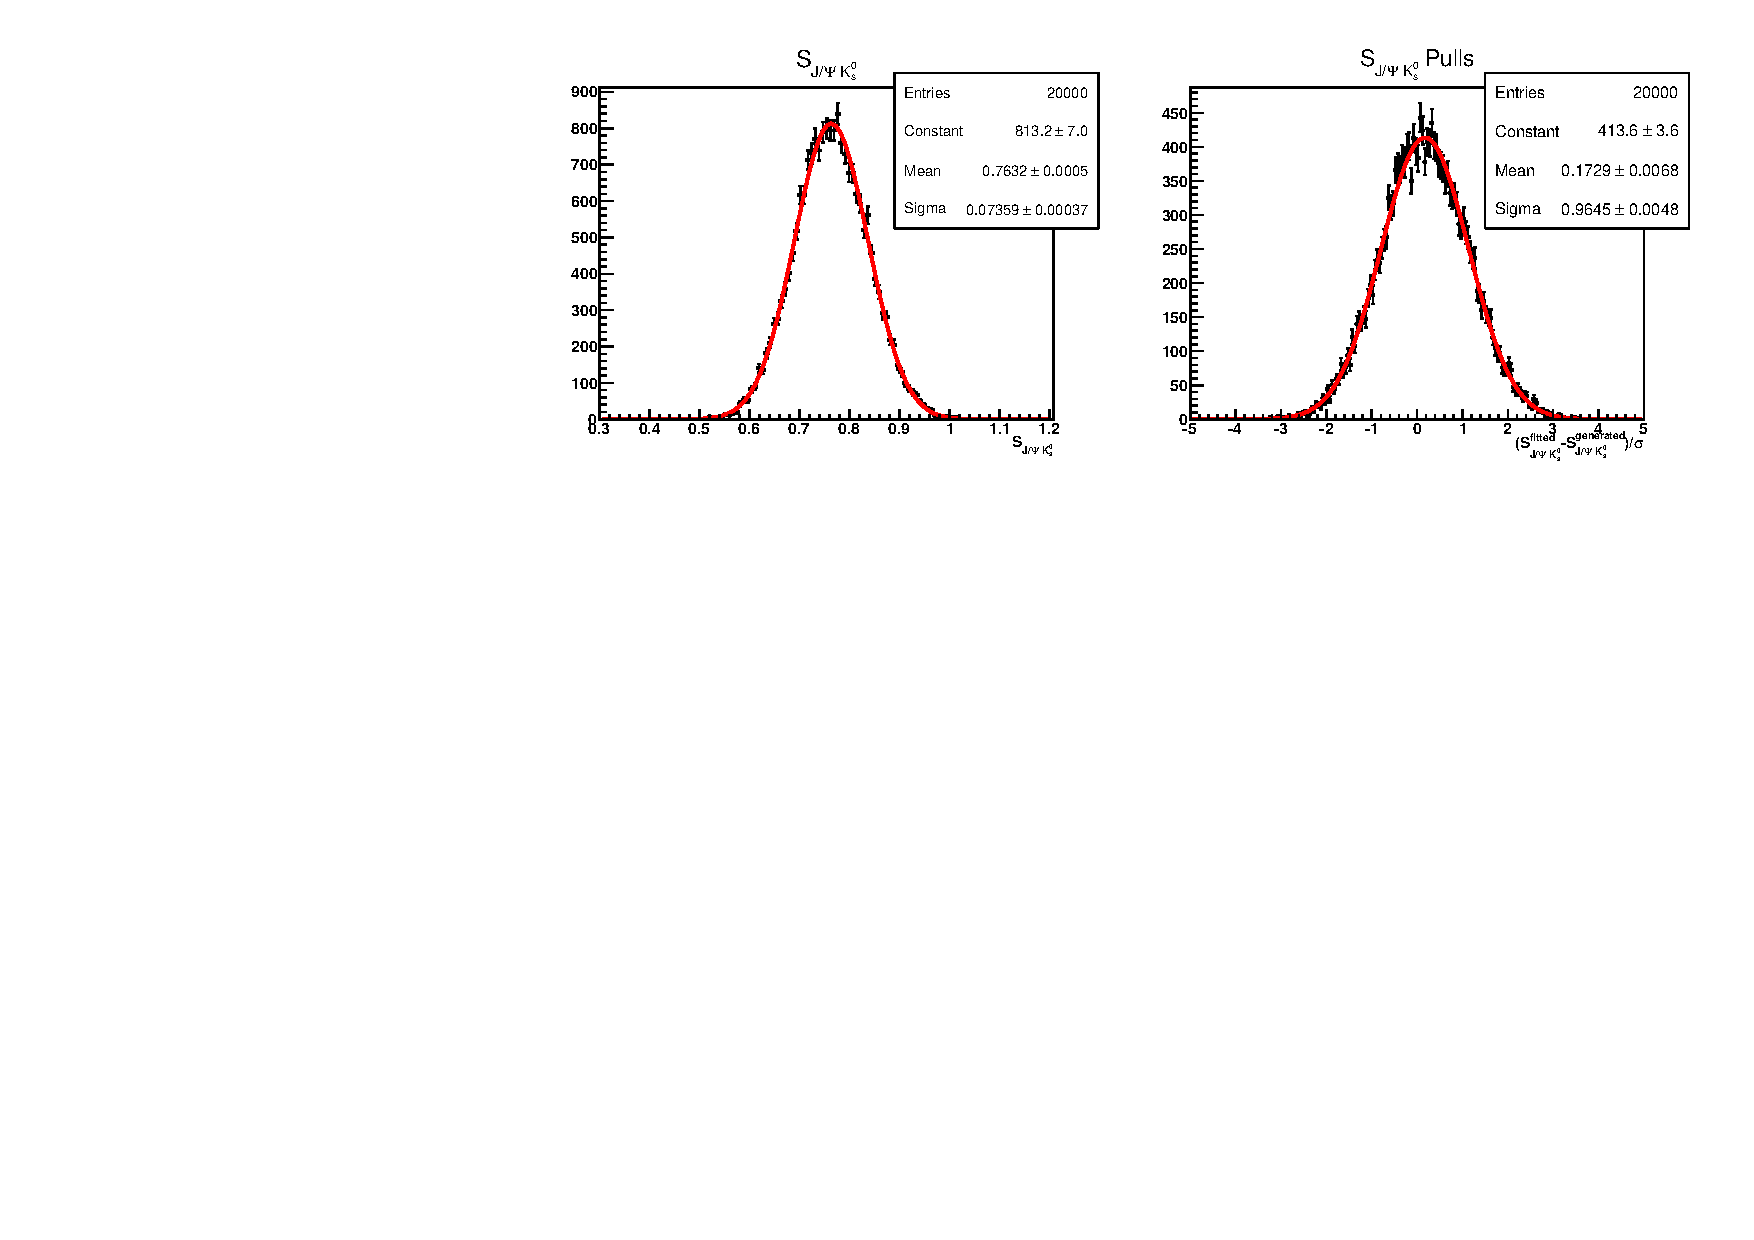
\includegraphics[width=0.75\textwidth]{tagging_calibration--}}
\subfigure[{$p_0 + \Delta p_0$,  $p_1 - \Delta p_1$}]{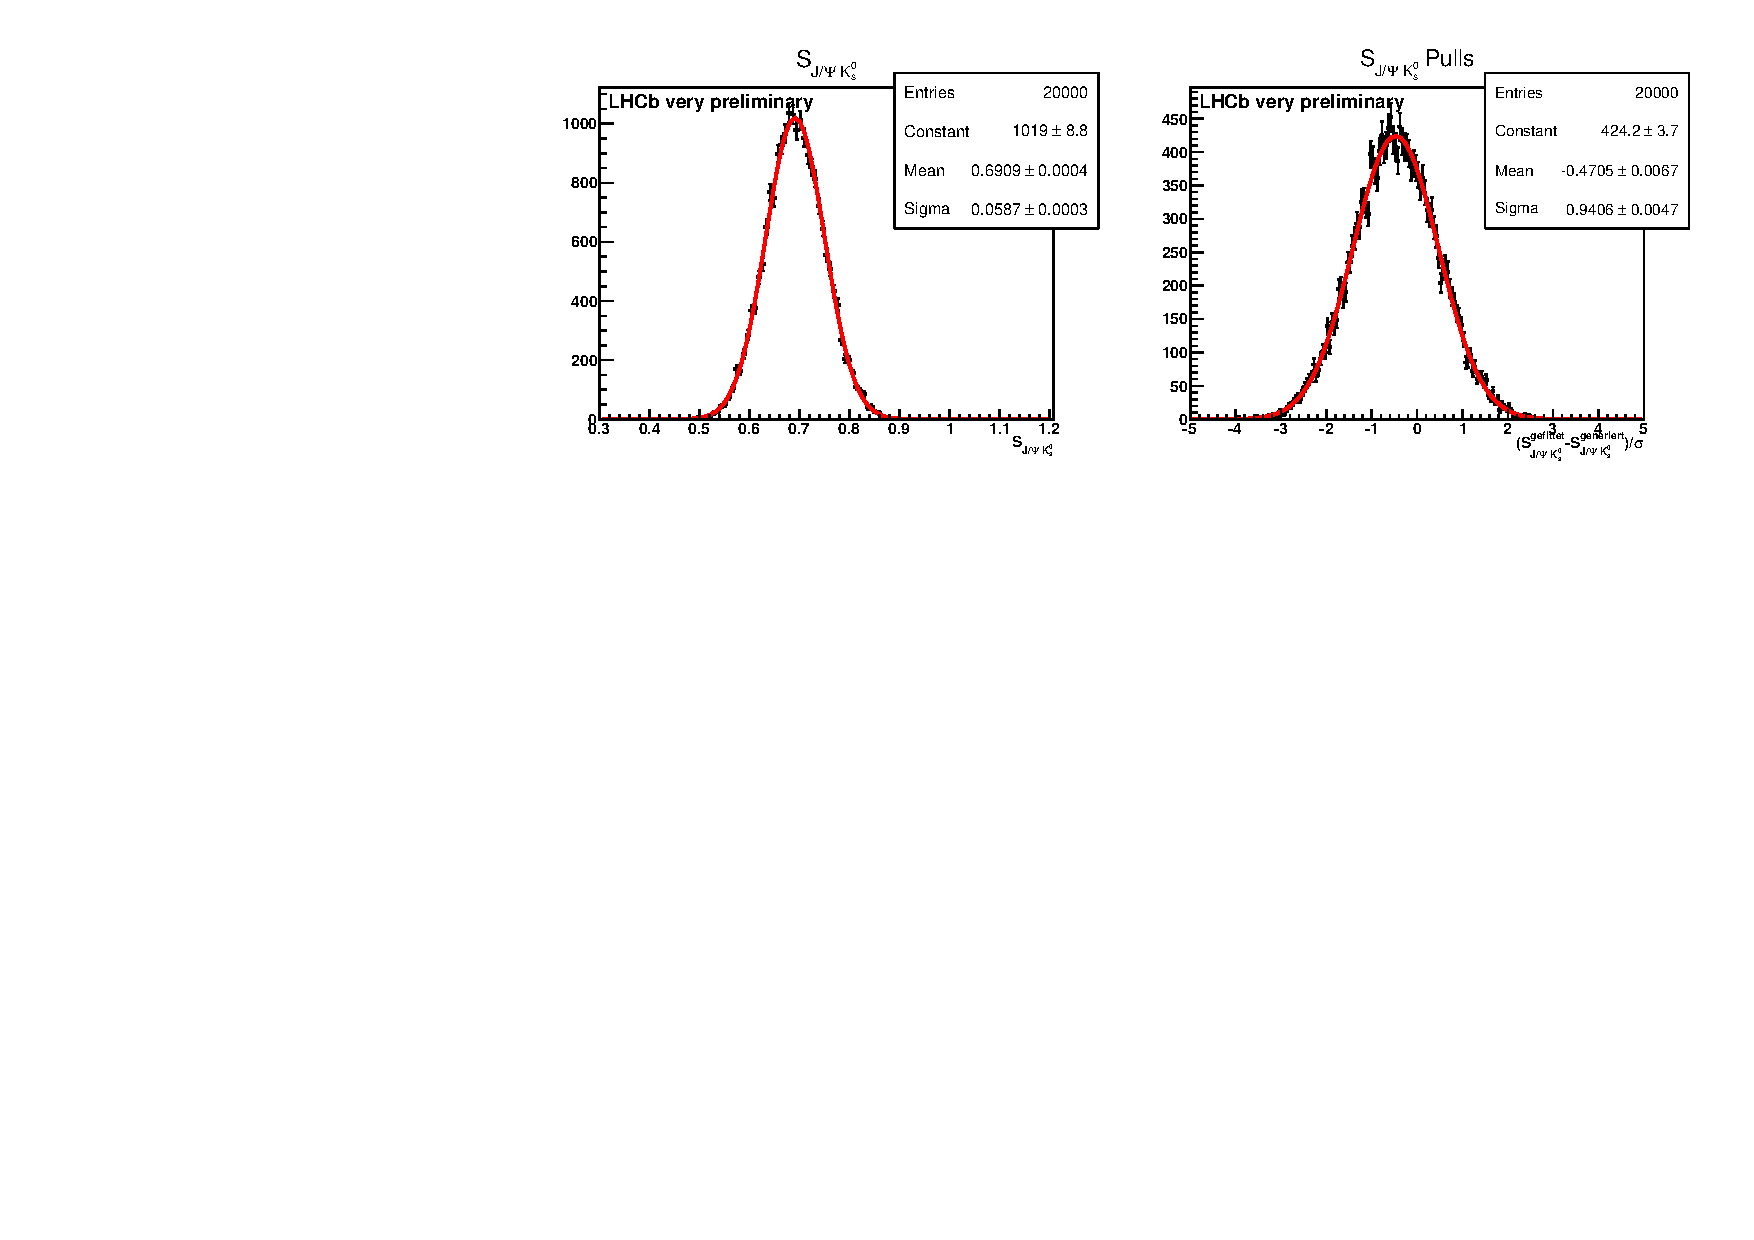
\includegraphics[width=0.75\textwidth]{tagging_calibration+-}}
\subfigure[{$p_0 - \Delta p_0$,  $p_1 + \Delta p_1$}]{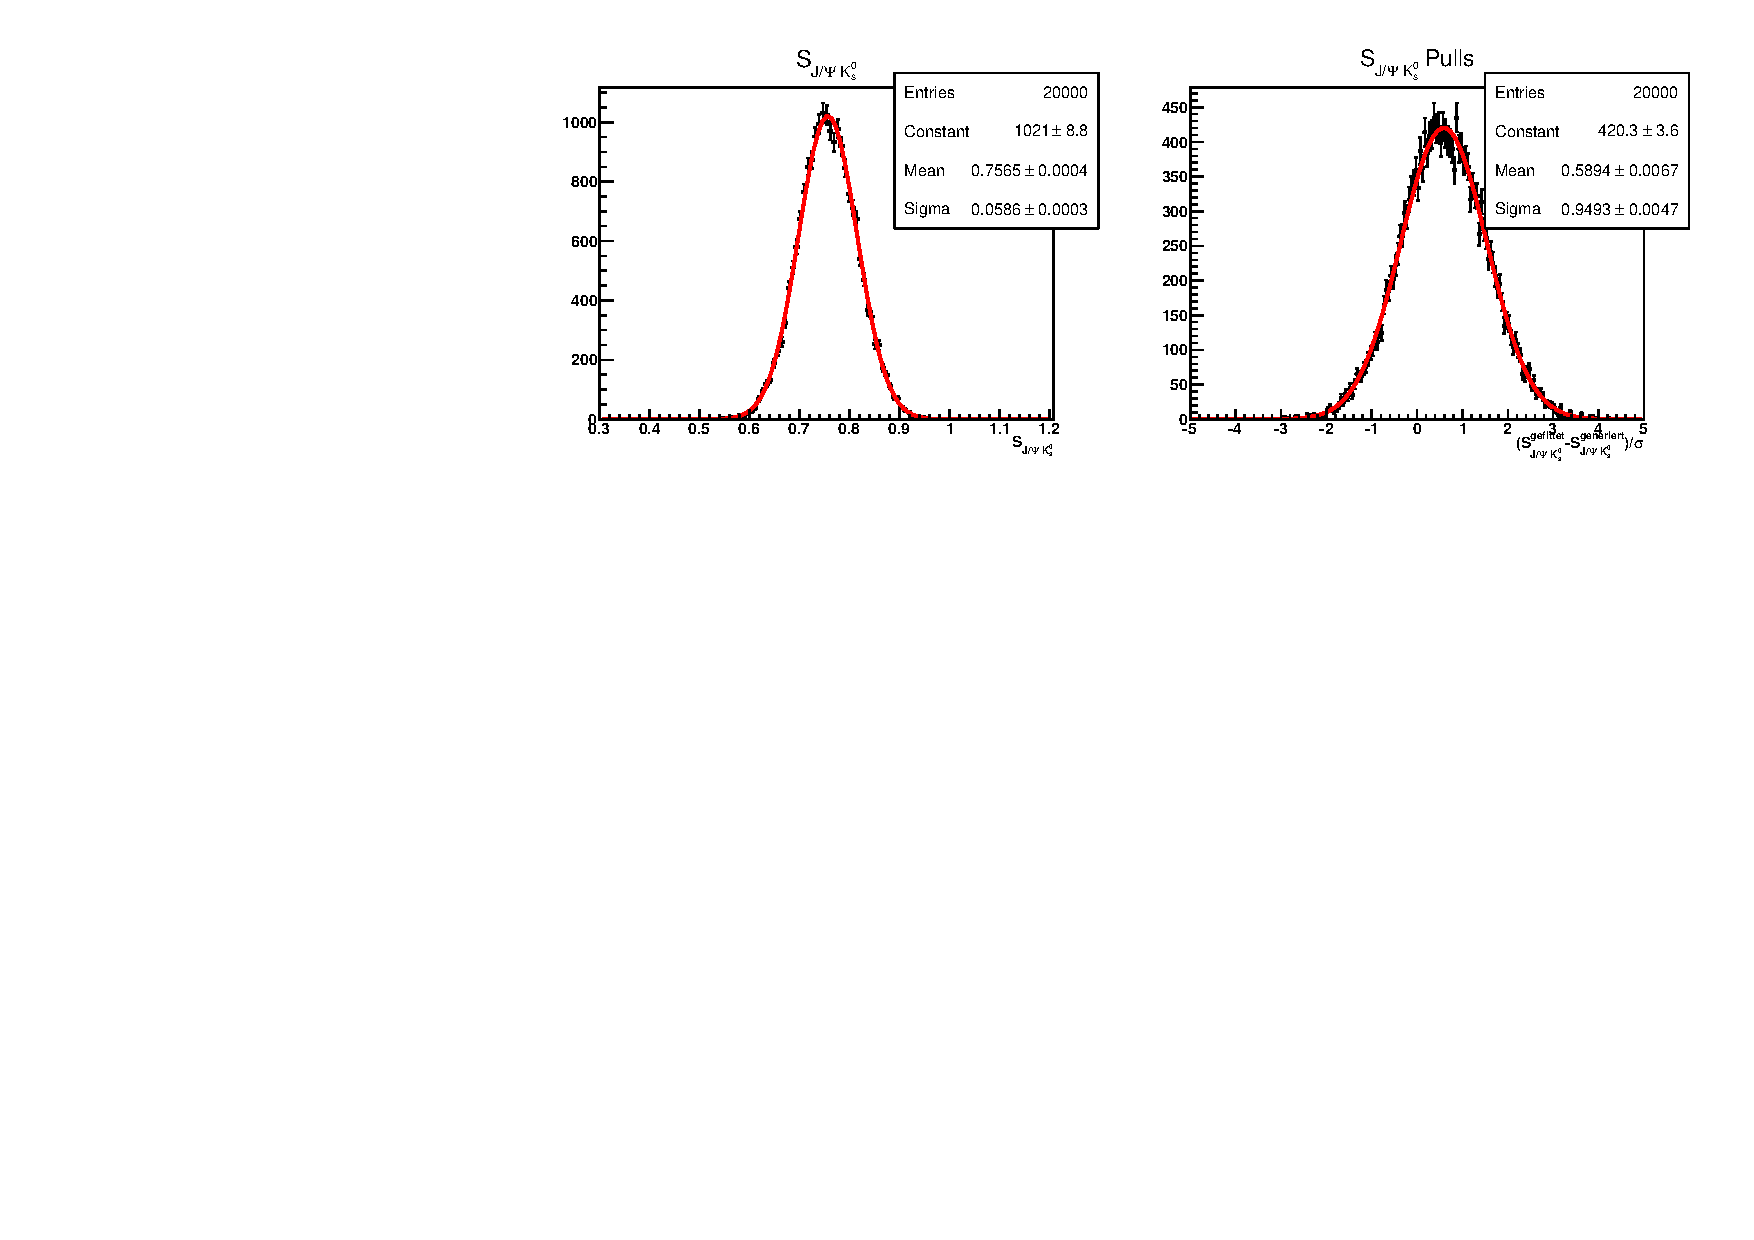
\includegraphics[width=0.75\textwidth]{tagging_calibration-+}}
\subfigure[{$p_0 + \Delta p_0$,  $p_1 + \Delta p_1$}]{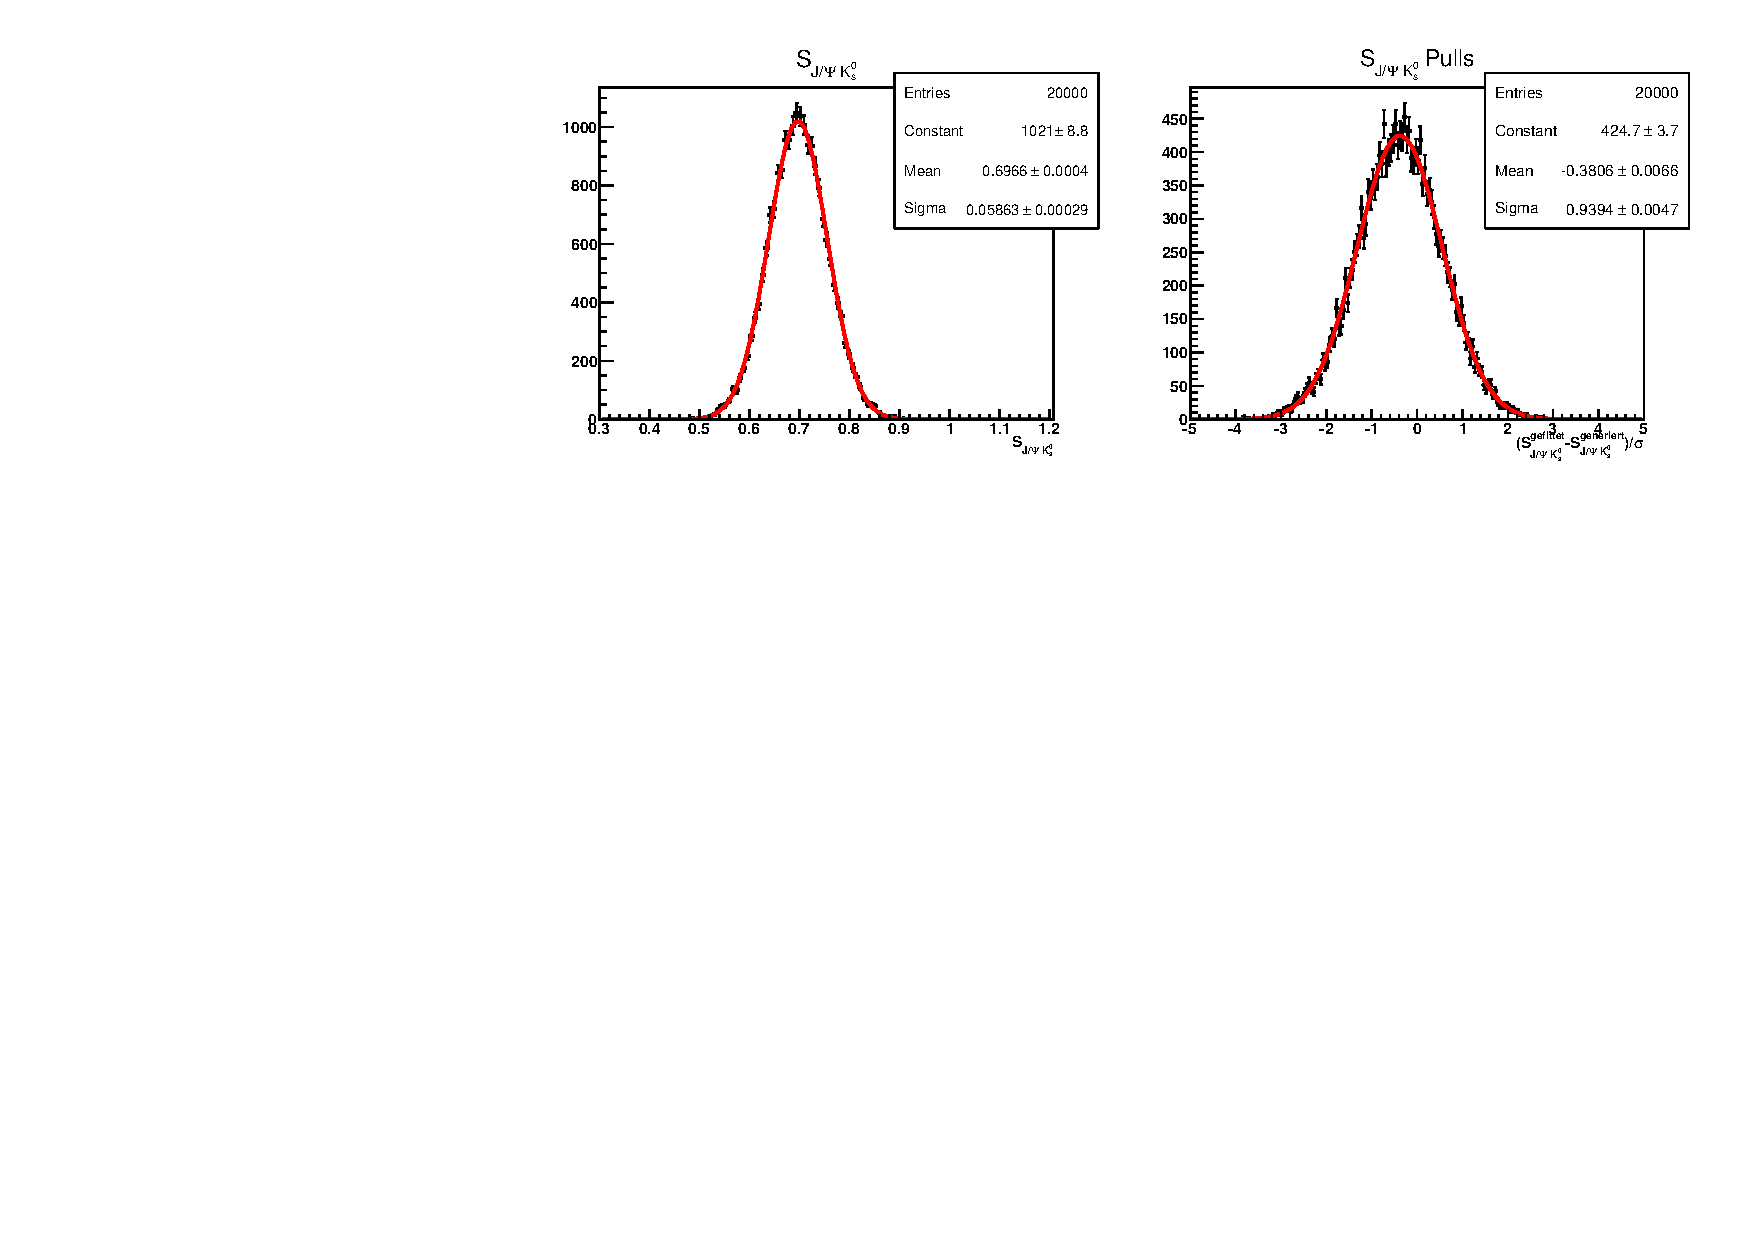
\includegraphics[width=0.75\textwidth]{tagging_calibration++}}
\caption{Toy MC Studie zur Abschätzung der Systematik durch die Tagging Kalibration. Bei der Generation wurden die Taggingparameter $p_0=0,382$ und $p_1=0,981$ um ihre systematischen Unsicherheiten $\Delta p_0 = 0,008$ bzw. $\Delta p_1 = 0,024$ variiert, der Fit wurde dann mit den ursprünglichen Werten $p_0$ und $p_1$ durchgeführt.}
\label{fig:toys_tag_calib}
\end{figure}

\section{Einfluss einer zeitabhängigen Akzeptanz} \label{kap:akzeptanz}
In der Analyse wurde der Einfluss einer zeitabhängigen Detektorakzeptanz vernachlässigt. Nimmt man an, dass sich die Akzeptanz von \Bd- und \Bdbar-Mesonen nicht unterscheiden, so hat die Akzeptanz keinen Einfluss auf die \CP-Asymmetrie nach Gleichung (\ref{eq:cp_asymm}), da sie sich hier herauskürzt. Beim Fit der Amplitude nach Gleichung (\ref{eq:fit_pdf}) ist dies aber nicht zwangsläufig der Fall. Um die Vernachlässigung einer zeitabhängigen Akzeptanz zu rechtfertigen, wird zunächst eine Bestimmung der Akzeptanz durchgeführt und anschließend mit einer Toy MC Studie ihr Einfluss überprüft.

\subsubsection{Bestimmung einer Akzeptanzfunktion} 
\Bd-Mesonen haben eine relativ lange Lebensdauer. Um sie von kurzlebigem Untergrund zu unterscheiden, befinden sich auf den Triggern und dem Stripping entsprechende Selektionen auf die Signifikanz der Zerfallslänge. Dies hat zur Folge, dass für kleine Flugzeiten ($t \lesssim 0,3\pico\second$) kaum \Bd-Mesonen im Detektor registriert werden. Es hat sich herausgestellt \cite{lhcb-paper}, dass dieser Effekt gut durch die Funktion
\begin{align}
\epsilon_1(t) = \frac{2}{\pi}\arctan[t\cdot \exp(at+b)]
\end{align}
parametrisiert werden kann. Je länger ein \Bd-Meson lebt, desto schwieriger wird es, diese Zerfallsprodukte im Detektor auf Grund seiner Geometrie nachzuweisen. Daher nimmt die Akzeptanz zu großen Zeiten hin wieder ab. Zur Parametrisierung fällt die Wahl auf eine lineare Funktion
\begin{align}
\epsilon_2(t) = 1 + \beta t \qquad (\beta < 0).
\end{align}
Die entsprechende gesamte Akzeptanzfunktion lautet demnach:
\begin{align}
\epsilon(t) = \epsilon_1(t) \cdot \epsilon_2(t) = \frac{2}{\pi}\arctan[t\cdot \exp(at+b)](1 + \beta t)
\end{align}
Zur Bestimmung der Parameter wird die Trennung von \Bd- und \Bdbar-Mesonen aufgehoben, sodass lediglich ein exponentieller Zerfall zu beobachten ist. Des weiteren wird die Selektion der Lebensdauer bei $0,3\pico\second$ nicht angewandt, sodass die Akzeptanz bei kleinen Eigenzeiten sichtbar wird. Die Wahrscheinlichkeitsdichtefunktion für den Fit lautet somit:
\begin{align}
\mathcal{P}_{acc}(t) \propto \epsilon(t)\cdot \e^{-t/\tau} = \e^{-t/\tau}\cdot\frac{2}{\pi}\arctan[t\cdot \exp(at+b)](1 + \beta t)
\end{align}
Die beiden Parameter $\tau$ und $\beta$ sind stark miteinander korreliert. Für eine geeignete Bestimmung der Parameter der Akzeptanz-Funktion wird daher die Lebensdauer auf den PDG-Wert $\tau = (1,519 \pm 0,007)\pico\second$ \cite{pdg-tau} gaußisch eingeschränkt, die anderen Parameter sind frei. Die Ergebnisse sind in Tabelle \ref{tab:fit_akzeptanz} aufgeführt, die entsprechenden Plots in Abbildung \ref{fig:fit_akzeptanz}. 
\begin{table}[hptb]
\centering
\caption{Ergebnis des Fits zur Bestimmung der zeitlichen Akzeptanz. $\tau$ wurde auf den PDG-Wert $\tau = (1,519 \pm 0,007)\pico\second$ \cite{pdg-tau} gaußisch eingeschränkt.}
\label{tab:fit_akzeptanz}
$\begin{array}{llr@{\pm}l}
\hline \hline 
\multicolumn{2}{l}{\text{Parameter}} & \multicolumn{2}{c}{\text{Ergebnis}}  \\ \hline
\tau  & [\ps]  &  1,519 & 0,007 \\
a   & [\ps]  &  47,9    & 5,6 \\
b   & &  -8,4    & 1,1 \\
\beta & [\ps^{-1}]  & -0,0090 & 0,0076 \\ 
\hline \hline
\end{array}$
\end{table}
\begin{figure}[hptb]
\centering
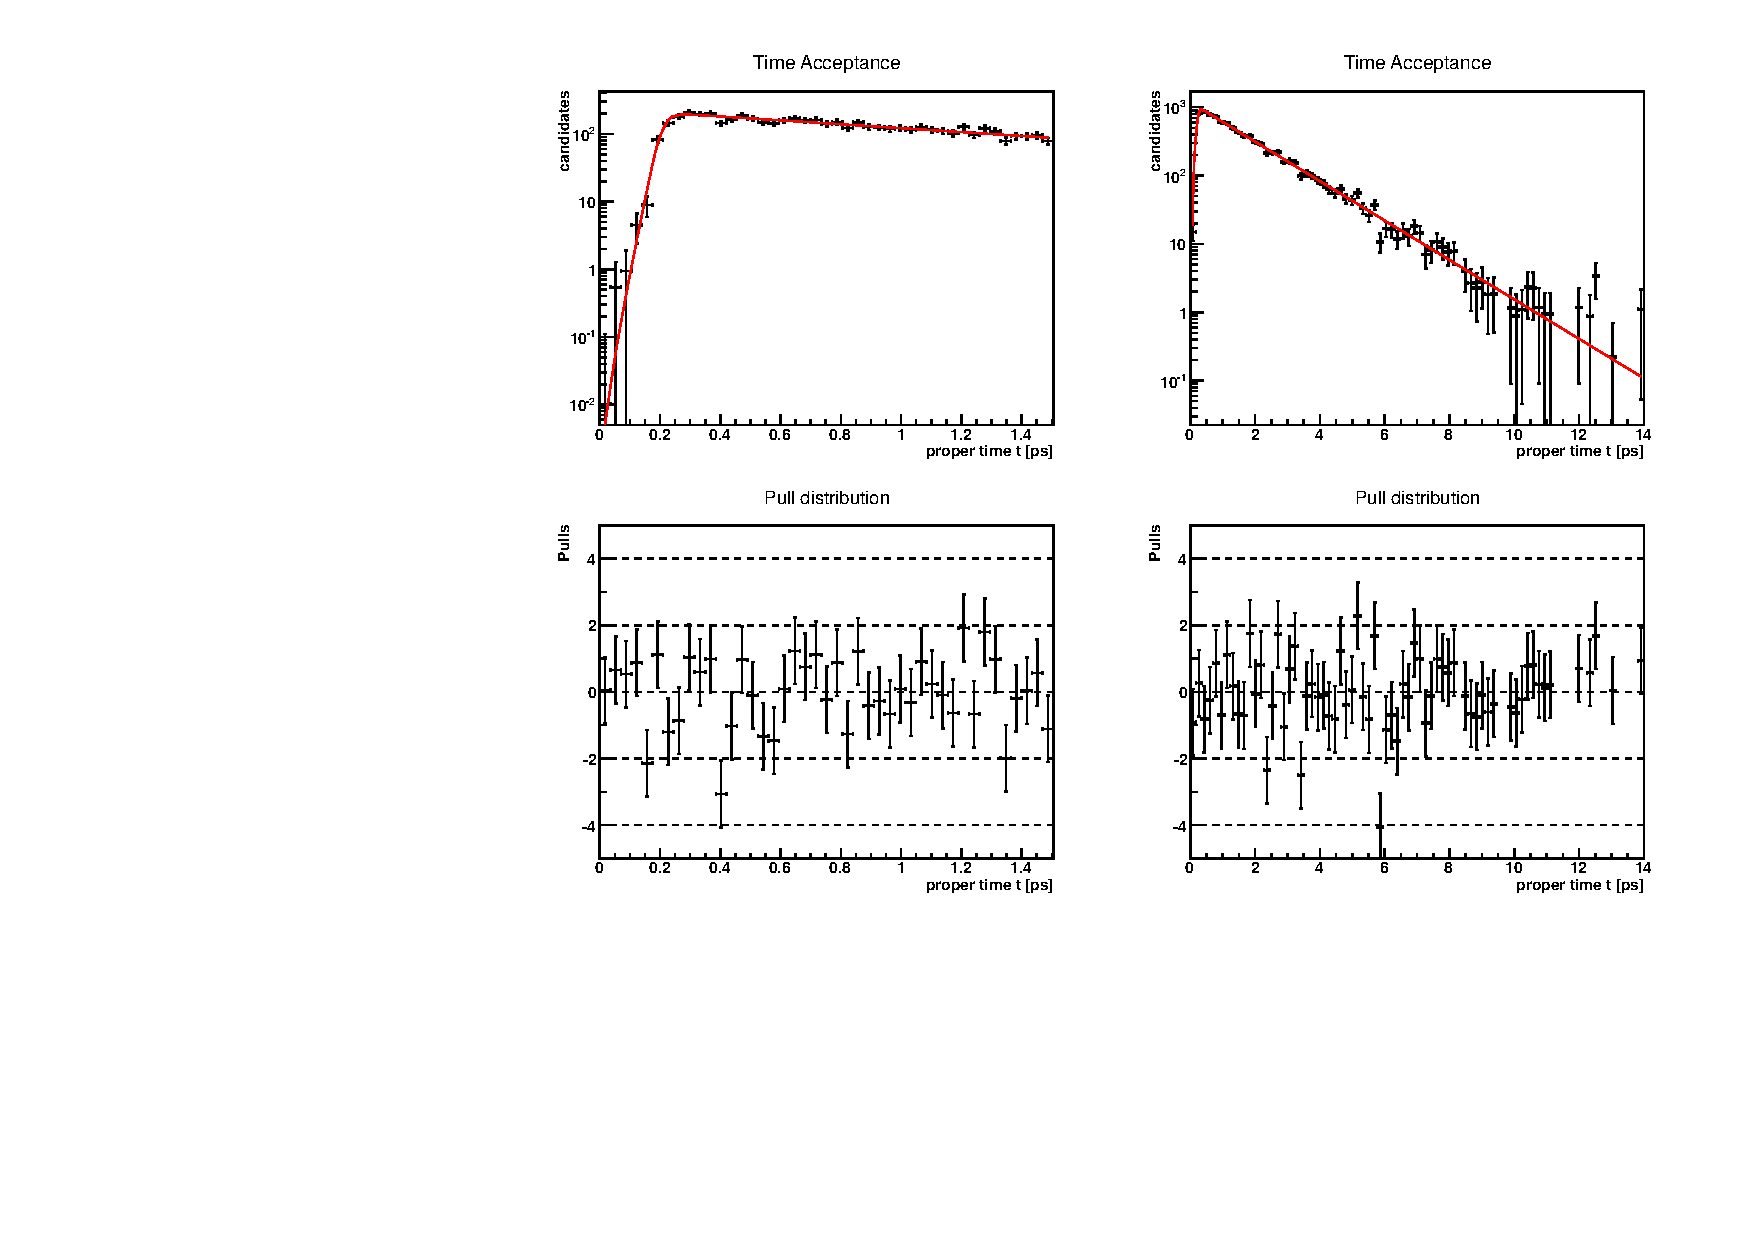
\includegraphics[width=\textwidth]{time_acceptance_fit}
\caption{Fit an die Eigenzeit-Verteilung aller \Bd-Mesonen mit eingeschlossener Akzeptanzfunktion (oben) sowie die entsprechende Pull-Verteilung (unten). Links: kurzlebiger Zeitbereich ($t<1,5\pico\second$), Rechts: gesamtes Eigenzeitspektrum ($0\ps < t < 14\ps$).}
\label{fig:fit_akzeptanz}
\end{figure}

\subsubsection{Bestimmung des Einflusses}
Durch die Selektion der Eigenzeit ab $t = 0,3\ps$ in der Datenselektion spielt die Akzeptanz für kleine Eigenzeiten kaum eine Rolle Dies wird dadurch deutlich, dass die Akzeptanzfunktion $\epsilon(0,3\ps) = 0,992$ und damit fast Eins ist. In der Analyse aus 2011 \cite{lhcb-paper} wurde nur ein geringer Effekt auf das Fitergebnis beobachtet. Dies soll nun verifiziert und das Vorgehen, im Eigenzeitfit die zeitliche Detektorakzeptanz zu vernachlässigen, gerechtfertigt werden. Mit den oben bestimmten Parametern wird die zeitliche Akzeptanz bei der Erzeugung von Daten einer weiteren Toy MC Studie berücksichtigt, der anschließende Fit aber ohne Akzeptanzfunktion durchgeführt. Die zur Erzeugung verwendeten Parameter entsprechen ansonsten denen in Kapitel \ref{kap:fit_bias}.
\begin{figure}[hptb]
\centering
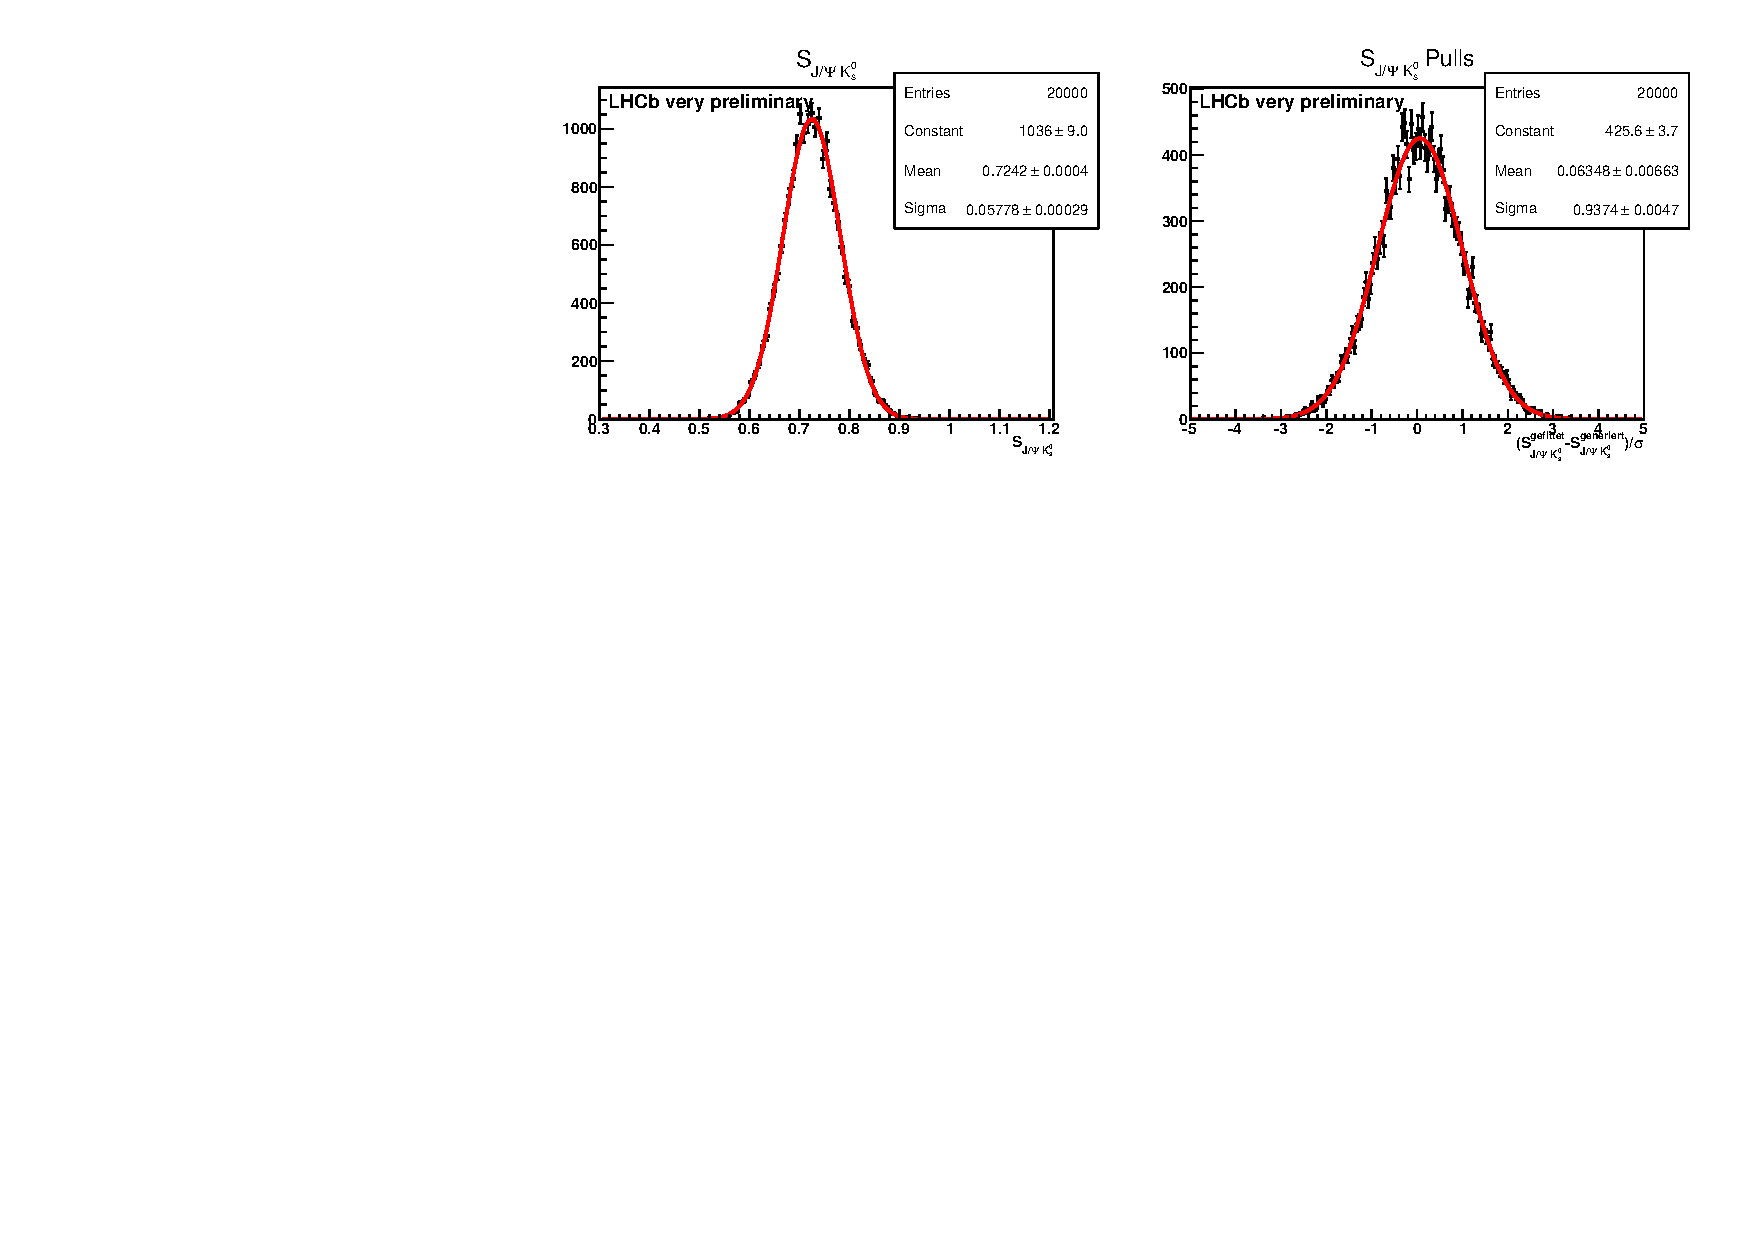
\includegraphics[width = \textwidth]{time_acceptance_toys}
\caption{Untersuchung des Einflusses einer zeitlichen Akzeptanz: Verteilung der aus der Toy MC Studie erhaltenen Amplituden $\SJPsi$ (links) sowie die dazugehörigen Pulls (rechts).}
\label{fig:toys_acceptance}
\end{figure}

Der Mittelwert der Amplitudenverteilung beträgt $\SJPsi = 0,72420 \pm 0,00041$. Die Abweichung vom Referenzwert $\SJPsi = 0,72343 \pm 0,00041$ (siehe Kap. \ref{kap:fit_bias}),
\begin{align}
\delta\SJPsi^{\text{Akz.}} = 0,00077\ ,
\end{align}
wird zur Abschätzung des Fehlers durch Vernachlässigung einer Akzeptanzfunktion verwendet. Gerade im Vergleich zum Einfluss des Flavour Taggings auf $\SJPsi$ ist dieser hier sehr gering. Somit erscheint das Vorgehen, keine Akzeptanz im Eigenzeitfit zu verwenden, gerechtfertigt.


\section{Korrelation zwischen Masse und Eigenzeit}
Die sFit-Methode funktioniert dann am besten, wenn das Signal und der Untergrund der Massenverteilung vollkommen unkorreliert zur Signal- und Untergrundverteilung der Eigenzeit ist. Es soll nun eine etwaige Korrelation zwischen Masse und Eigenzeit untersucht und der Einfluss auf $\SJPsi$ festgestellt werden. Dazu wird die Massenverteilung in vier verschiedenen Zeitbereichen gefittet, die Tabelle \ref{tab:mass_ct} zu entnehmen sind. Anschließend wird die gesamte Eigenzeitverteilung gefittet, dabei werden aber die Massenparameter auf die in den 4 Massenfits erhaltenen Werte fixiert. Die Ergebnisse des jeweiligen Fits sind ebenfalls in Tabelle \ref{tab:mass_ct} aufgeführt.
\begin{table}[hptb]
\centering
\caption{Einteilung der Eigenzeitbereiche sowie Fitresultate für $\SJPsi$ bei Fixierung der Masse auf die in den Zeitbereichen enthaltene Massenform. Weiterhin werden die Abweichung $\Delta\SJPsi$ vom regulären Datenfit und der Signalanzahl $N_{sig}$ eines jeden Eigenzeitbereichs genannt.}
\label{tab:mass_ct}
\begin{tabular}{c l r@{$\pm$}l c c}
\hline \hline
Nr. & Eigenzeitfenster des Massenfits & \multicolumn{2}{c}{$\SJPsi$} & $\Delta\SJPsi$ & $N_{sig}$\\ \hline
1 & $t \in [0,3; 0,7] \pico\second$ & 0,5318 & 0,0626 & -0,0029 & 2882 \\
2 & $t \in [0,7; 1,5] \pico\second$ & 0,5361 & 0,0625 & 0,0014 & 4066 \\
3 & $t \in [1,5; 3] \pico\second$ & 0,5361 & 0,0625 & 0,0014 & 4230 \\
4 & $t \in [3; 14] \pico\second$ & 0,5353 & 0,0624 & 0,0006 & 2177 \\ \hline \hline
\end{tabular}
\end{table}

Zur Abschätzung des Fehlers werden zunächst die Abweichungen $\Delta\SJPsi$ vom (noch verdeckten) Referenzwert aus dem regulären Eigenzeitfit $\SJPsi = 0,5347 \pm 0,0626$ berechnet (siehe Kap. \ref{kap:fitergebnis}) und diese dann - gewichtet nach der Signalzahl $N_{sig}$ eines jeden Bereichs - quadratisch gemittelt:
\begin{align}
\delta\SJPsi^{m/t} = \sqrt{\frac{\sum N_i (\Delta\SJPsi)_i^2}{\sum N_i}} = 0,0018
\end{align}

\section{Eigenzeitauflösung} \label{kap:aufloesung}
Bei einer effektiven Eigenzeitauflösung von $\sigma_{\text{eff}} = (0,0665 \pm 0,0013)\ps$ im Vergleich zur \Bd-Oszillationsfrequenz $\Delta m_d = (0,521 \pm 0.039)\ps$ erwartet man keine nennenswerten Effekte auf die Amplitude $\SJPsi$. Um überhaupt einen Effekt zu sehen, werden die Auflösungsparameter $\sigma_i$ um 20\% ihres Werte erhöht bzw. gesenkt und damit dann der Datensatz gefittet. Die größte Abweichung vom Referenzwert des regulären Eigenzeitfits wird als systematischer Fehler angenommen. Die Ergebnisse finden sich in Tabelle \ref{tab:syst_resolution}.

\begin{table}[hptb]
\centering
\caption{Ergebnisse des Eigenzeitfits bei Variaton der Auflösungsparameter $\sigma_i$ um $\pm 20\%$.}
\label{tab:syst_resolution}
\begin{tabular}{l c c c r@{$\pm$}l r }
\hline \hline
Variation & $\sigma_1$ & $\sigma_2$ & $\sigma_3$ & \multicolumn{2}{c}{$\SJPsi$} & $\Delta\SJPsi$ \\ \hline
$+20\%$ & 0,576 & 0,05275 & 0,1118 & 0,5351 & 0,0626 & 0,0004 \\
$-20\%$ & 0,384 & 0,03517 & 0,0746 & 0,5345 & 0,0625 & -0,0002 \\ \hline \hline
\end{tabular}
\end{table}
Es zeigt sich, dass eine exakte Bestimmung der Auflösung nicht von Nöten ist, da sie im Vergleich zu anderen Systematiken vor allem gegenüber der Flavour Tagging Kalibration vernachlässigt werden kann. Dennoch wird ein sytematischer Fehler durch die Auflösung mit
\begin{align}
\delta\SJPsi^{\text{Res.}} = 0,0004
\end{align}
assoziiert.

\section{Gesamtsystematik}
Tabelle \ref{tab:syst_gesamt} fasst nochmals alle systematischen Unsicherheiten zusammen. Der Gesamtfehler wird durch quadratische Addition berechnet.
\begin{table}[hptb]
\centering
\caption{Zusammenfassung der systematischen Unsicherheiten}
\label{tab:syst_gesamt}
\begin{tabular}{l c }
\hline \hline
Effekt & $\delta\SJPsi$ \\ \hline
Fitmethode & 0,0033 \\
Flavour Tagging Kalibration & 0,0331 \\
Eigenzeitakzeptanz & 0,0008 \\
Korrelation Masse $\leftrightarrow$ Eigenzeit & 0,0018 \\ 
Eigenzeitauflösung & 0,0004 \\ \hline 
Gesamt & 0,0333 \\ \hline \hline
\end{tabular}
\end{table}

Es ist deutlich zu erkennen, dass die Kalibration der Flavour Tagging Algorithmen die dominierende Systematik ist. Obwohl hier zur Abschätzung der Systematik Werte der 2011-Kalibration genommen werden mussten, wird sich an dieser Tatsache nicht viel ändern, sobald diese Untersuchung mit Werten aus 2012 wiederholt wurde. Der systematische Fehler von $\delta\SJPsi^{\text{stat.}}=0,0333$ ist nur etwa halb so groß wie der statistische $\delta\SJPsi^{\text{syst.}}=0,0626$. Damit ist definitiv noch Potential da, die Präzision durch mehr Datennahme zu verbessern. Zudem ist auch zu erwarten, dass die systematischen Unsicherheiten der Flavour Tagging Kalibration mit mehr Daten ebenfalls reduziert wird.

\chapter{Zusammenfassung}

\begin{thebibliography}{---}
\bibitem{lhcb-paper} LHCb-Analyse, ...
\bibitem{kleinknecht}  K. Kleinknecht, Uncovering ...
\bibitem{pdg-tau} PDG-Wert für Tau \\ \url{http://pdglive.lbl.gov/popupblockdata.brl?nodein=S042T&inscript=Y&fsizein=1&clumpin0=} (Stand: 02.07.2013)
\end{thebibliography}

\printglossaries 
% Selbstständigkeitserklärung
\chapter*{Erklärung}

Ich versichere, dass ich diese Arbeit selbstständig verfasst und keine anderen als die angegebenen Quellen und Hilfsmittel benutzt habe. \\
\vspace{0.2cm}
\begin{flushleft}
Heidelberg, den 19.08.2013,\\
\vspace{2cm}
%Unterschrift
Patrick Fahner
\end{flushleft}


\end{document}


